% !TeX program = xelatex
\documentclass[a4paper,10pt]{article}

% ============================================================================
% កញ្ចប់សម្ភារៈសិក្សាបោះពុម្ព ស-ខ្មៅ (Printable Classroom Materials - Grade 8 3.1 INEQ1)
% ត្រូវគ្នា ១០០% នឹង LS_Plan_INEQ1.tex និង Teaching_Scenario_INEQ1.tex
% ============================================================================
\usepackage[a4paper, left=1.0cm, right=1.0cm, top=0.75cm, bottom=1.05cm, footskip=0.55cm]{geometry}
\usepackage{amsmath, amssymb}
\usepackage{unicode-math}
\usepackage{fontspec}
\usepackage{array, colortbl}
\usepackage[table]{xcolor}
\usepackage{enumitem}
\usepackage{pifont}
\usepackage{fancyhdr}
\usepackage{lastpage}
\usepackage{tikz}
\usepackage[most]{tcolorbox}
\usetikzlibrary{calc, arrows.meta, angles, quotes, decorations.markings, positioning, babel}

% LaTeX 2025 compatibility guard
\makeatletter
\let\@expl@@@mark@update@singlecol@structures@@\relax
\makeatother

% ============================================================================
% ការកំណត់ពុម្ពអក្សរផ្លូវការ (Word-Styled Khmer + Cambria Math + Times New Roman)
% ============================================================================
% Cross-platform font path resolver (Windows local + Linux/Cloud repo fonts/)
\providecommand{\NGSFindFonts}{%
  \IfFileExists{C:/Windows/Fonts/cambria.ttc}{%
    \def\NGSSysPath{C:/Windows/Fonts/}%
    \def\NGSUserPath{C:/Users/KIT/AppData/Local/Microsoft/Windows/Fonts/}%
  }{%
    \IfFileExists{./fonts/KhmerOSsiemreap.ttf}{\def\NGSSysPath{./fonts/}\def\NGSUserPath{./fonts/}}{%
    \IfFileExists{../fonts/KhmerOSsiemreap.ttf}{\def\NGSSysPath{../fonts/}\def\NGSUserPath{../fonts/}}{%
    \IfFileExists{../../fonts/KhmerOSsiemreap.ttf}{\def\NGSSysPath{../../fonts/}\def\NGSUserPath{../../fonts/}}{%
    \IfFileExists{../../../fonts/KhmerOSsiemreap.ttf}{\def\NGSSysPath{../../../fonts/}\def\NGSUserPath{../../../fonts/}}{%
    \IfFileExists{../../../../fonts/KhmerOSsiemreap.ttf}{\def\NGSSysPath{../../../../fonts/}\def\NGSUserPath{../../../../fonts/}}{%
    \IfFileExists{../../../../../fonts/KhmerOSsiemreap.ttf}{\def\NGSSysPath{../../../../../fonts/}\def\NGSUserPath{../../../../../fonts/}}{%
    \IfFileExists{../../../../../../fonts/KhmerOSsiemreap.ttf}{\def\NGSSysPath{../../../../../../fonts/}\def\NGSUserPath{../../../../../../fonts/}}{%
      \def\NGSSysPath{../../../../../../../fonts/}\def\NGSUserPath{../../../../../../../fonts/}%
    }}}}}}}%
  }%
}
\NGSFindFonts

\setmathfont[
  Path={\NGSSysPath},
  FontIndex=1,
  Scale=1.02
]{cambria.ttc}

\defaultfontfeatures{Ligatures=TeX}

\setmainfont[
  Path={\NGSUserPath},
  Extension=.ttf,
  Script=Khmer,
  BoldFont={KhmerOSsiemreap},
  BoldFeatures={FakeBold=1.8},
  ItalicFont={KhmerOSsiemreap},
  ItalicFeatures={FakeSlant=0.25},
  BoldItalicFont={KhmerOSsiemreap},
  BoldItalicFeatures={FakeBold=1.8, FakeSlant=0.25}
]{KhmerOSsiemreap}

\newfontfamily\muol[
  Path={\NGSUserPath},
  Extension=.ttf,
  Script=Khmer
]{KhmerOSmuollight}

\newfontfamily\TimesEn[
  Path={\NGSSysPath},
  Extension=.ttf,
  BoldFont={timesbd},
  ItalicFont={timesi},
  BoldItalicFont={timesbi}
]{times}

\newfontfamily\CalibriFont[
  Path={\NGSSysPath},
  Extension=.ttf
]{calibri}

\newfontfamily\Tacteing[
  Path={\NGSUserPath}
]{TACTENG.TTF}

\XeTeXlinebreaklocale "km"
\XeTeXlinebreakskip = 0pt plus 1pt minus 0.1pt

% ============================================================================
% ក្ដារពណ៌ ស-ខ្មៅ សុទ្ធសម្រាប់ការបោះពុម្ព (Strict Monochrome Print Palette)
% ============================================================================
\definecolor{panelgray}{gray}{0.92} % ~gray!8
\definecolor{headgray}{gray}{0.85}  % ~gray!15
\definecolor{midgray}{gray}{0.75}   % ~gray!25
\definecolor{darkline}{gray}{0.35}  % ~gray!65

\pagestyle{fancy}
\fancyhf{}
\renewcommand{\headrulewidth}{0pt}
\fancyfoot[L]{\fontsize{7.8pt}{10pt}\selectfont អនុវិទ្យាល័យព្រះក្រសាំង \en{---} គណិតវិទ្យា ថ្នាក់ទី៨ \en{|} មេរៀនទី១២ (៣.១) វិសមភាពជ្រុង-មុំ (ស-ខ្មៅ) \en{|} ថ្ងៃព្រហស្បតិ៍ ៩រោច កត្តិក ២៥៧០ \en{|} ថ្ងៃទី៣ ខែធ្នូ ឆ្នាំ២០២៦}
\fancyfoot[R]{\fontsize{8.2pt}{10pt}\selectfont ទំព័រ \en{\thepage\ / \pageref{LastPage}}}

\setlength{\parindent}{0pt}
\setlength{\parskip}{0pt}
\setlength{\tabcolsep}{4pt}

% ============================================================================
% ម៉ាក្រូជំនួយ (Helper Macros)
% ============================================================================
\newcommand{\en}[1]{{\TimesEn #1}}
\newcommand{\enbf}[1]{{\TimesEn\bfseries #1}}
\newcommand{\unit}[1]{\,\text{\en{#1}}}
\newcommand{\cnum}[1]{\mbox{\fontsize{10pt}{12pt}\selectfont\ding{\numexpr181+#1\relax}}}
\newcommand{\scissors}{\ding{34}}
\newcommand{\chkbox}{\tikz[baseline=-0.15ex]\draw[black, line width=0.85pt] (0,0) rectangle (0.24cm,0.24cm);}
\newcommand{\tickslash}{\tikz[baseline=-0.2ex]\draw[black, line width=1.1pt] (0,0) -- (0.12cm,0.22cm);}
\newcommand{\tri}[1]{\ensuremath{\triangle #1}}
\newcommand{\ang}[1]{\ensuremath{\angle #1}}
\newcommand{\khmflourish}{{\Tacteing\fontsize{32pt}{13pt}\selectfont\raisebox{-4pt}{3}}}

\newcommand{\pagebanner}[2]{%
  \begin{tcolorbox}[
    enhanced, sharp corners, colback=headgray, colframe=black,
    boxrule=1.1pt, boxsep=1pt, top=3pt, bottom=3pt, left=6pt, right=6pt,
    after skip=4pt
  ]
    {\muol\fontsize{9.1pt}{13.5pt}\selectfont #1}\hfill{\fontsize{8.0pt}{11.5pt}\selectfont\textbf{#2}}
  \end{tcolorbox}%
}

\newcolumntype{L}[1]{>{\raggedright\arraybackslash}p{#1}}
\newcolumntype{C}[1]{>{\centering\arraybackslash}p{#1}}

% Bold B&W Tick marks (>=1.0pt print safe)
\tikzset{
  tk1/.style={postaction={decorate},decoration={markings,
    mark=at position 0.50 with {\draw[black, line width=1.05pt] (0,-0.11)--(0,0.11);}}},
  tk2/.style={postaction={decorate},decoration={markings,
    mark=at position 0.44 with {\draw[black, line width=1.05pt] (0,-0.11)--(0,0.11);},
    mark=at position 0.56 with {\draw[black, line width=1.05pt] (0,-0.11)--(0,0.11);}}},
  tkslash/.style={postaction={decorate},decoration={markings,
    mark=at position 0.50 with {\draw[black, line width=1.05pt] (-0.07,-0.10)--(0.07,0.10);}}},
  tkslashR/.style={postaction={decorate},decoration={markings,
    mark=at position 0.50 with {\draw[black, line width=1.05pt] (-0.07,0.10)--(0.07,-0.10);}}}
}

\begin{document}
\fontsize{9.0pt}{13.2pt}\selectfont

% ============================================================================
% ទំព័រទី ១៖ សម្ភារៈ E2 ខ្នាតពិត 1:1 (បត់/កាត់ ΔABC + បន្ទះរំកិល 4.00 cm + POE 2A-2B)
% ============================================================================
\pagebanner{សម្ភារៈទី ១៖ បន្ទះកាត់ \enbf{E2} ខ្នាតពិត \enbf{1:1} វិសមភាពជ្រុង\enbf{-}មុំ \enbf{\&} ពិសោធន៍ \enbf{POE 2A--2B}}{ទំព័រ ១/៦ \en{-- E2 Explore}}

% --- ប្រអប់ព្រមានខ្នាតពិត & បន្ទះផ្ទៀង 5.00 cm (x=1cm, y=1cm) ---
\noindent
\begin{minipage}[c]{11.9cm}
  \begin{tcolorbox}[
    enhanced, sharp corners, colback=panelgray, colframe=black,
    boxrule=1.0pt, boxsep=1pt, top=3pt, bottom=3pt, left=6pt, right=6pt
  ]
    \fontsize{8.0pt}{11.2pt}\selectfont
    \textbf{ការណែនាំសំខាន់មុនបោះពុម្ព (\en{Print at 100\% / Actual Size})៖} ត្រូវជ្រើស \textbf{\en{Scale: Actual Size 100\%}} \en{--} \textbf{ហាម \en{Fit to Page}} ដើម្បីឱ្យ $\tri{ABC}$ ($4.00\text{--}5.50\text{--}6.50\unit{cm}$), បន្ទះរំកិល $AD=AB=4.00\unit{cm}$, \en{POE 2A} ($30^\circ\text{--}60^\circ\text{--}90^\circ$) និង \en{POE 2B} ត្រូវខ្នាតពិត \en{1:1}។\\[1.5pt]
    \textbf{ក្រុមអ្នកបច្ចេកទេសដងស្ទូច និងទ្វារបត់មុំ៖} កាត់ \scissors{} រំកិលបន្ទះ $AD=AB$ ដៅ $D$ លើ $AC$ បត់ផ្នត់ $BD$ និងវាស់ផ្ទៀងដោយបន្ទាត់ \en{cm}។
  \end{tcolorbox}
\end{minipage}%
\hfill
\begin{minipage}[c]{6.8cm}
  \begin{tcolorbox}[
    enhanced, sharp corners, colback=white, colframe=black,
    boxrule=1.0pt, boxsep=1pt, top=2.5pt, bottom=2.5pt, left=4pt, right=4pt
  ]
    \centering
    {\fontsize{7.7pt}{9.8pt}\selectfont\textbf{បន្ទះផ្ទៀងខ្នាតពិត \en{5.00 cm} (\en{Actual Size 100\%})}}\\[1.5pt]
    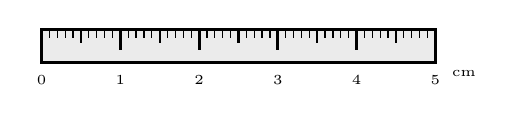
\begin{tikzpicture}[x=1cm, y=1cm, every node/.style={font=\scriptsize, text=black}]
      \draw[black, line width=1.1pt, fill=panelgray] (0,0) rectangle (5.0, 0.42);
      \foreach \m in {0,...,50}{
        \pgfmathsetmacro{\xval}{\m*0.1}
        \draw[black, line width=0.45pt] (\xval, 0.42) -- (\xval, 0.31);
      }
      \foreach \h in {0,0.5,...,5.0}{
        \draw[black, line width=0.8pt] (\h, 0.42) -- (\h, 0.24);
      }
      \foreach \c in {0,1,2,3,4,5}{
        \draw[black, line width=1.1pt] (\c, 0.42) -- (\c, 0.15);
        \node[below=1pt, font=\tiny] at (\c, 0.0) {\en{\c}};
      }
      \node[right=2pt, font=\tiny] at (5.02, -0.14) {\en{cm}};
    \end{tikzpicture}
  \end{tcolorbox}
\end{minipage}

\vspace{5pt}

% --- ផ្នែកទី ១៖ សកម្មភាព 1 — កាត់/បត់ ∆ABC សាមញ្ញ (1:1) + បន្ទះរំកិល 4.00 cm (1:1) ---
\textbf{១. សកម្មភាព \en{1} ៖ កាត់/បត់ $\tri{ABC}$ (\en{4.00--5.50--6.50 cm}) និងបន្ទះរំកិល $AD=AB=4.00\unit{cm}$ (\en{x=1cm, y=1cm})}

\vspace{3pt}
\noindent
\begin{minipage}[c]{7.70cm}
  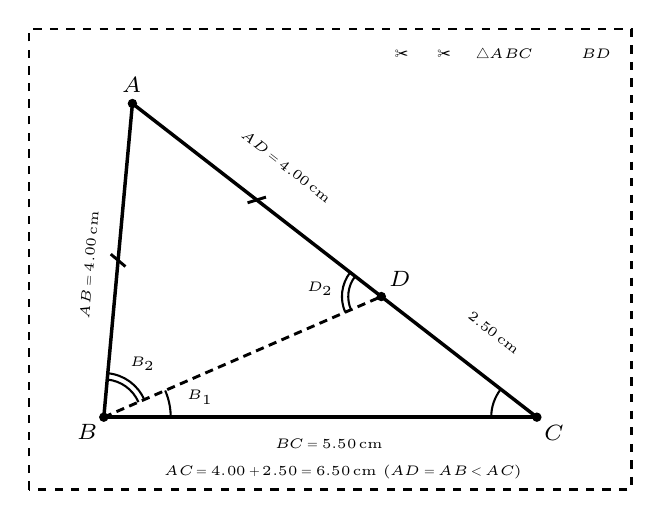
\begin{tikzpicture}[x=1cm, y=1cm, every node/.style={font=\scriptsize, text=black}]
    % Cuttable box: 7.65 cm x 5.85 cm
    \draw[black, dashed, line width=0.95pt] (0, 0) rectangle (7.65, 5.85);
    \node[anchor=north east, font=\tiny] at (7.52, 5.73) {\scissors\ \textbf{កាត់ \scissors{} តាម $\tri{ABC}$ និងបត់តាម $BD$}};

    % Exact 1:1 Scalene ABC shifted by (+0.95, +0.92):
    % B=(0,0), C=(5.5,0), A=(0.3636, 3.9834), D=(3.5245, 1.5321)
    \coordinate (B) at (0.9500, 0.9200);
    \coordinate (C) at (6.4500, 0.9200);
    \coordinate (A) at (1.3136, 4.9034);
    \coordinate (D) at (4.4745, 2.4521);

    % Triangle edges (solid cut line) & dashed crease BD
    \draw[black, line width=1.25pt] (B) -- (C);
    \draw[black, line width=1.25pt, tkslash] (A) -- (B);
    \draw[black, line width=1.25pt, tkslash] (A) -- (D);
    \draw[black, line width=1.25pt] (D) -- (C);
    \draw[black, densely dashed, line width=1.05pt] (B) -- (D);

    % Distinct angle arcs: B2 (double), B1 (single), D2 (double), C (single)
    \pic[draw=black, line width=0.75pt, angle radius=4.8mm]{angle=D--B--A};
    \pic[draw=black, line width=0.75pt, angle radius=5.6mm]{angle=D--B--A};
    \pic[draw=black, line width=0.75pt, angle radius=8.5mm]{angle=C--B--D};
    \pic[draw=black, line width=0.75pt, angle radius=4.2mm]{angle=A--D--B};
    \pic[draw=black, line width=0.75pt, angle radius=5.0mm]{angle=A--D--B};
    \pic[draw=black, line width=0.75pt, angle radius=5.8mm]{angle=A--C--B};

    % Angle labels placed cleanly on bisectors away from segments/arcs
    \node[fill=white, inner sep=0.7pt, font=\tiny] at ($(B)+(54.1:0.84)$) {$B_2$};
    \node[fill=white, inner sep=0.7pt, font=\tiny] at ($(B)+(11.7:1.25)$) {$B_1$};
    \node[fill=white, inner sep=0.7pt, font=\tiny] at ($(D)+(172.9:0.78)$) {$D_2$};

    % Vertices & clean exterior labels
    \fill[black] (A) circle (0.06) node[above=3pt, fill=white, inner sep=0.8pt, font=\footnotesize] {$A$};
    \fill[black] (B) circle (0.06) node[below left=2.5pt, fill=white, inner sep=0.8pt, font=\footnotesize] {$B$};
    \fill[black] (C) circle (0.06) node[below right=2.5pt, fill=white, inner sep=0.8pt, font=\footnotesize] {$C$};
    \fill[black] (D) circle (0.06) node[above right=2.5pt and 2pt, fill=white, inner sep=0.8pt, font=\footnotesize] {$D$};

    % Side length annotations strictly outside triangle segments (0 collisions!)
    \node[font=\tiny, rotate=85, fill=white, inner sep=0.6pt] at ($(A)!0.52!(B)+(-0.36, 0.02)$) {$AB=4.00\unit{cm}$};
    \node[font=\tiny, fill=white, inner sep=0.6pt] at ($(B)!0.52!(C)+(0, -0.34)$) {$BC=5.50\unit{cm}$};
    \node[font=\tiny, rotate=-38, fill=white, inner sep=0.6pt] at ($(A)!0.48!(D)+(0.44, 0.38)$) {$AD=4.00\unit{cm}$};
    \node[font=\tiny, rotate=-38, fill=white, inner sep=0.6pt] at ($(D)!0.52!(C)+(0.40, 0.34)$) {$2.50\unit{cm}$};
    \node[font=\tiny, fill=white, inner sep=0.6pt] at (3.85, 0.22) {សរុប $AC = 4.00 + 2.50 = 6.50\unit{cm}$ ($AD=AB<AC$)};
  \end{tikzpicture}
\end{minipage}%
\hfill
\begin{minipage}[c]{11.05cm}
  % Top row: 1:1 Cut-out Notched Slider Strip (4.00 cm exact) + Quick guide
  \noindent
  \begin{minipage}[c]{5.55cm}
    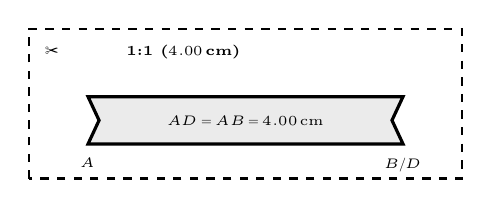
\begin{tikzpicture}[x=1cm, y=1cm, every node/.style={font=\scriptsize, text=black}]
      \draw[black, dashed, line width=0.95pt] (0, 0) rectangle (5.50, 1.90);
      \node[anchor=north west, font=\tiny] at (0.08, 1.82) {\scissors\ \textbf{កាត់បន្ទះរំកិល \en{1:1} ($4.00\unit{cm}$)}};
      % Exact 4.00 cm notched bar from x=0.75 to x=4.75
      \draw[black, line width=1.15pt, fill=panelgray]
        (0.75, 0.44) -- (4.75, 0.44) -- (4.61, 0.74) -- (4.75, 1.04) --
        (0.75, 1.04) -- (0.89, 0.74) -- cycle;
      \node[font=\tiny, fill=panelgray, inner sep=0.8pt] at (2.75, 0.74) {$AD = AB = 4.00\unit{cm}$};
      \node[below=1pt, font=\tiny] at (0.75, 0.42) {$A$};
      \node[below=1pt, font=\tiny] at (4.75, 0.42) {$B / D$};
    \end{tikzpicture}
  \end{minipage}%
  \hfill
  \begin{minipage}[c]{5.35cm}
    \begin{tcolorbox}[
      enhanced, sharp corners, colback=panelgray, colframe=black,
      boxrule=0.85pt, boxsep=1pt, top=3pt, bottom=3pt, left=4.5pt, right=4.5pt
    ]
      \raggedright\fontsize{7.3pt}{10.2pt}\selectfont
      \textbf{ជំហានរំកិល និងបត់ (\en{1:1})៖}\\
      \textbf{១.} កាត់បន្ទះ $AD=AB=4.00\unit{cm}$ រំកិលលើ $AC$ ពី $A \to D$។\\
      \textbf{២.} ព្រោះ $AD=4.00 < AC=6.50$ ចំណុច $D$ ស្ថិត\textbf{ចន្លោះ} $A, C$។\\
      \textbf{៣.} បត់ផ្នត់ $BD$ រួចពិនិត្យ $\ang{B_2}, \ang{D_2}, \ang{C}$!
    \end{tcolorbox}
  \end{minipage}

  \vspace{4pt}
  % Bottom row: Act 1 Record Box
  \begin{tcolorbox}[
    enhanced, sharp corners, colback=white, colframe=black,
    boxrule=1.0pt, boxsep=1pt, top=4pt, bottom=4pt, left=5pt, right=5pt,
    title={\textbf{កំណត់ត្រាសកម្មភាព \en{1} ($AC > AB \Rightarrow \ang{B} > \ang{C}$)}},
    colbacktitle=headgray, coltitle=black, fonttitle=\fontsize{8.0pt}{10.8pt}\selectfont
  ]
    \raggedright\fontsize{7.6pt}{11.0pt}\selectfont
    $\bullet$ $AD = AB = 4.00\unit{cm} \Rightarrow \tri{ABD}$ \textbf{សមបាទ}កំពូល $A \Rightarrow \ang{B_2} = \ang{\underline{\hspace{0.45cm}}}$ ($61.3^\circ$)\quad\chkbox\\[2pt]
    $\bullet$ $\ang{D_2}$ ជា\textbf{មុំក្រៅ}នៃ $\tri{BCD} \Rightarrow \ang{D_2} = \ang{B_1} + \ang{C} \Rightarrow \ang{D_2} > \ang{\underline{\hspace{0.45cm}}}$ ($37.8^\circ$)\quad\chkbox\\[2pt]
    $\bullet$ បន្ថែមមុំ៖ $\ang{B} = \ang{B_1} + \ang{B_2} > \ang{B_2} = \ang{D_2} > \ang{C} \Rightarrow \ang{B} \underline{\hspace{0.45cm}} \ang{C}$ ($84.8^\circ > 37.8^\circ$)\quad\chkbox
  \end{tcolorbox}
\end{minipage}

\vspace{6pt}

% --- ផ្នែកទី ២៖ សកម្មភាព 2 (Dual POE 1:1, x=1cm, y=1cm) ---
\textbf{២. សកម្មភាព \en{2} (\en{POE 2A \& 2B}) ៖ អន្ទាក់ផលធៀបលីនេអ៊ែរ និងអន្ទាក់ត្រីកោណ ២ ផ្សេងគ្នា (\en{x=1cm, y=1cm})}

\vspace{3pt}
\noindent
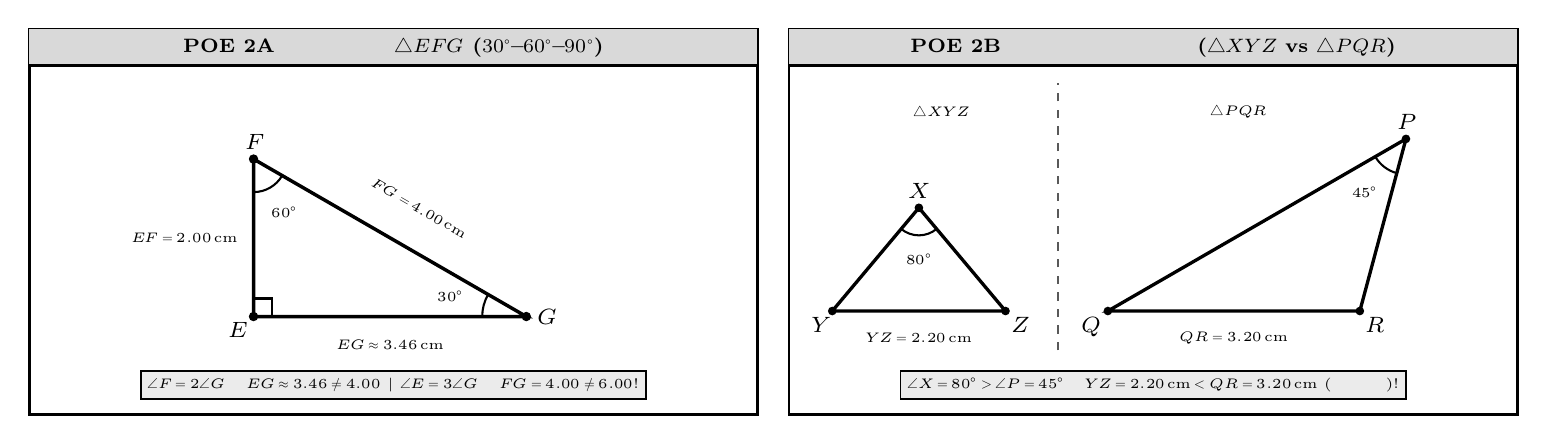
\begin{tikzpicture}[x=1cm, y=1cm, every node/.style={font=\scriptsize, text=black}]
  % === Panel POE 2A: Exact 30-60-90 1:1 right triangle EFG ===
  \begin{scope}[shift={(0,0)}]
    \draw[black, line width=1.05pt] (0, 0) rectangle (9.25, 4.90);
    \fill[headgray] (0, 4.44) rectangle (9.25, 4.90);
    \draw[black, line width=0.85pt] (0, 4.44) -- (9.25, 4.44);
    \node[font=\scriptsize] at (4.625, 4.67) {\textbf{\en{POE 2A}៖ អន្ទាក់គុណលីនេអ៊ែរ $\tri{EFG}$ ($30^\circ\text{--}60^\circ\text{--}90^\circ$)}};

    \coordinate (E) at (2.8500, 1.2500);
    \coordinate (G) at (6.3141, 1.2500);
    \coordinate (F) at (2.8500, 3.2500);

    \draw[black, line width=1.25pt] (E) -- (G) -- (F) -- cycle;
    \pic[draw=black, line width=0.8pt, angle radius=2.3mm]{right angle=G--E--F};
    \pic[draw=black, line width=0.75pt, angle radius=4.2mm]{angle=E--F--G};
    \pic[draw=black, line width=0.75pt, angle radius=5.6mm]{angle=F--G--E};

    \node[fill=white, inner sep=0.6pt, font=\tiny] at ($(F)+(-60:0.78)$) {$60^\circ$};
    \node[fill=white, inner sep=0.6pt, font=\tiny] at ($(G)+(165:1.00)$) {$30^\circ$};

    \fill[black] (E) circle (0.06) node[below left=2pt, fill=white, inner sep=0.7pt, font=\footnotesize] {$E$};
    \fill[black] (F) circle (0.06) node[above=2.5pt, fill=white, inner sep=0.7pt, font=\footnotesize] {$F$};
    \fill[black] (G) circle (0.06) node[right=3pt, fill=white, inner sep=0.7pt, font=\footnotesize] {$G$};

    \node[font=\tiny, fill=white, inner sep=0.7pt] at ($(E)!0.50!(F)+(-0.88, 0)$) {$EF=2.00\unit{cm}$};
    \node[font=\tiny, fill=white, inner sep=0.7pt] at ($(E)!0.50!(G)+(0, -0.36)$) {$EG\approx 3.46\unit{cm}$};
    \node[font=\tiny, rotate=-30, fill=white, inner sep=0.7pt] at ($(F)!0.48!(G)+(0.44, 0.34)$) {$FG=4.00\unit{cm}$};

    \node[font=\tiny, fill=panelgray, draw=black, line width=0.6pt, inner sep=2.5pt] at (4.625, 0.38) {$\ang{F}=2\ang{G}$ តែ $EG\approx 3.46\neq 4.00$ \en{|} $\ang{E}=3\ang{G}$ តែ $FG=4.00\neq 6.00$!};
  \end{scope}

  % === Panel POE 2B: Two-Separate-Triangles Trap (1:1) ===
  \begin{scope}[shift={(9.65,0)}]
    \draw[black, line width=1.05pt] (0, 0) rectangle (9.25, 4.90);
    \fill[headgray] (0, 4.44) rectangle (9.25, 4.90);
    \draw[black, line width=0.85pt] (0, 4.44) -- (9.25, 4.44);
    \node[font=\scriptsize] at (4.625, 4.67) {\textbf{\en{POE 2B}៖ អន្ទាក់ឆ្លងត្រីកោណ ២ ដាច់ពីគ្នា ($\tri{XYZ}$ \en{vs} $\tri{PQR}$)}};

    \coordinate (Y) at (0.5500, 1.3200);
    \coordinate (Z) at (2.7500, 1.3200);
    \coordinate (X) at (1.6500, 2.6309);
    \draw[black, line width=1.2pt] (Y) -- (Z) -- (X) -- cycle;
    \pic[draw=black, line width=0.75pt, angle radius=3.5mm]{angle=Y--X--Z};
    \node[fill=white, inner sep=0.5pt, font=\tiny] at ($(X)+(-90:0.65)$) {$80^\circ$};
    \fill[black] (X) circle (0.055) node[above=2.5pt, fill=white, inner sep=0.6pt, font=\footnotesize] {$X$};
    \fill[black] (Y) circle (0.055) node[below left=2pt, fill=white, inner sep=0.6pt, font=\footnotesize] {$Y$};
    \fill[black] (Z) circle (0.055) node[below right=2pt, fill=white, inner sep=0.6pt, font=\footnotesize] {$Z$};
    \node[font=\tiny, fill=white, inner sep=0.7pt] at ($(Y)!0.50!(Z)+(0, -0.34)$) {$YZ=2.20\unit{cm}$};
    \node[font=\tiny] at (1.65, 3.85) {\textbf{ត្រីកោណតូច $\tri{XYZ}$}};

    \draw[darkline, dashed, line width=0.75pt] (3.42, 0.82) -- (3.42, 4.22);

    \coordinate (Q) at (4.0500, 1.3200);
    \coordinate (R) at (7.2500, 1.3200);
    \coordinate (P) at (7.8356, 3.5056);
    \draw[black, line width=1.2pt] (Q) -- (R) -- (P) -- cycle;
    \pic[draw=black, line width=0.75pt, angle radius=4.5mm]{angle=Q--P--R};
    \node[fill=white, inner sep=0.5pt, font=\tiny] at ($(P)+(-127.5:0.86)$) {$45^\circ$};
    \fill[black] (P) circle (0.055) node[above=2.5pt, fill=white, inner sep=0.6pt, font=\footnotesize] {$P$};
    \fill[black] (Q) circle (0.055) node[below left=2pt, fill=white, inner sep=0.6pt, font=\footnotesize] {$Q$};
    \fill[black] (R) circle (0.055) node[below right=2pt, fill=white, inner sep=0.6pt, font=\footnotesize] {$R$};
    \node[font=\tiny, fill=white, inner sep=0.7pt] at ($(Q)!0.50!(R)+(0, -0.34)$) {$QR=3.20\unit{cm}$};
    \node[font=\tiny] at (5.45, 3.85) {\textbf{ត្រីកោណធំ $\tri{PQR}$}};

    \node[font=\tiny, fill=panelgray, draw=black, line width=0.6pt, inner sep=2.5pt] at (4.625, 0.38) {$\ang{X}=80^\circ > \ang{P}=45^\circ$ តែ $YZ=2.20\unit{cm} < QR=3.20\unit{cm}$ (គ្មានស្ពានស្មើ)!};
  \end{scope}
\end{tikzpicture}

\vspace{6pt}

% --- តារាង POE (Predict - Observe - Explain) ---
\begin{tcolorbox}[
  enhanced, sharp corners, colback=white, colframe=black,
  boxrule=1.0pt, boxsep=1pt, top=5pt, bottom=5pt, left=6pt, right=6pt
]
  \raggedright\fontsize{8.0pt}{11.6pt}\selectfont
  \textbf{\en{P} -- ទស្សន៍ទាយមុនវាស់ (\en{Predict})៖}\\[3pt]
  \textbf{១)} ក្នុង $\tri{EFG}$៖ បើ $\ang{F}=2\ang{G}$ ($60^\circ=2\times 30^\circ$) និង $\ang{E}=3\ang{G}$ ($90^\circ=3\times 30^\circ$) តើ $EG=2EF$ និង $FG=3EF$ ឬទេ? \quad\chkbox~បាទ/ចាស \quad\chkbox~ទេ\\[3pt]
  \textbf{២)} រវាង $\tri{XYZ}$ និង $\tri{PQR}$៖ បើ $\ang{X}=80^\circ > \ang{P}=45^\circ$ តើ $YZ > QR$ ឬទេ? \quad\chkbox~បាទ/ចាស \quad\chkbox~ទេ\\[5pt]

  \textbf{\en{O} -- តារាងវាស់ផ្ទៀងខ្នាតពិត \en{1:1} ដោយបន្ទាត់ \en{cm} (\en{Observe})៖}\\[3pt]
  \renewcommand{\arraystretch}{1.22}
  \begin{tabular}{|L{4.20cm}|L{9.10cm}|L{4.00cm}|}
    \hline
    \cellcolor{headgray}\textbf{ផ្ទាំងពិសោធន៍ \en{POE}} & \cellcolor{headgray}\textbf{រង្វាស់ខ្នាតពិត \en{1:1} (\en{cm}) និងការប្រៀបធៀប} & \cellcolor{headgray}\textbf{លទ្ធផលពិសោធន៍} \\ \hline
    \textbf{\en{POE 2A}}៖ $\tri{EFG}$ ($30^\circ\text{--}60^\circ\text{--}90^\circ$) & $EF=\underline{\hspace{0.55cm}}\unit{cm},\; EG=\underline{\hspace{0.55cm}}\unit{cm},\; FG=\underline{\hspace{0.55cm}}\unit{cm}$ \newline ពិនិត្យផលធៀប៖ $EG \stackrel{?}{=} 2EF$ (\chkbox~ស្មើ \chkbox~មិនស្មើ) \en{|} $FG \stackrel{?}{=} 3EF$ (\chkbox~ស្មើ \chkbox~មិនស្មើ) & លំដាប់៖ $FG > EG > EF$ \newline ផលធៀប៖ \chkbox~មិនមែន $\times 2, \times 3$! \\ \hline
    \textbf{\en{POE 2B}}៖ $\tri{XYZ}$ \en{vs} $\tri{PQR}$ & $YZ=\underline{\hspace{0.55cm}}\unit{cm}$ (ឈម $80^\circ$) \en{|} $QR=\underline{\hspace{0.55cm}}\unit{cm}$ (ឈម $45^\circ$) & \chkbox~$YZ < QR$ (ទោះ $80^\circ > 45^\circ$!) \\ \hline
  \end{tabular}\\[5pt]

  \textbf{\en{E} -- ពន្យល់សន្និដ្ឋាន (\en{Explain})៖} ទ្រឹស្ដីបទវិសមភាពជ្រុង-មុំ \textbf{រក្សាបានតែលំដាប់ ($<, >$)} ប៉ុន្តែ \textbf{មិនរក្សាផលធៀបគុណ} ឡើយ ហើយប្រើបានតែក្នុង\textbf{ត្រីកោណតែមួយ} (លើកលែងតែមានស្ពានអង្កត់ស្មើភ្ជាប់)៖ $\underline{\hspace{4.2cm}}$
\end{tcolorbox}

\clearpage

% ============================================================================
% ទំព័រទី ២៖ E4 Elaborate — ២ ប័ណ្ណ "លំហាត់គំរូ (ទំ.១៥៨–១៥៩)" + តារាងអក្សរឈមបាត់
% ============================================================================
\pagebanner{សម្ភារៈទី ២៖ កាត \enbf{E4} «ផែនទីសមីការមុំក្នុង \enbf{180} ដឺក្រេ និងក្បួនអក្សរឈមបាត់»}{ទំព័រ ២/៦ \en{-- E4 Elaborate} (កាត់ ២ ប័ណ្ណ \scissors)}

\newcommand{\eFourCardINEQ}[1]{%
\begin{tcolorbox}[
  enhanced, sharp corners, colback=white, colframe=white,
  borderline={1.0pt}{0pt}{black, dashed},
  boxsep=1pt, top=5pt, bottom=5pt, left=5.5pt, right=5.5pt
]
  \begin{tcolorbox}[
    enhanced, sharp corners, colback=headgray, colframe=black,
    boxrule=0.8pt, boxsep=1pt, top=3pt, bottom=3pt, left=5pt, right=5pt, after skip=5pt
  ]
    \fontsize{8.3pt}{11.2pt}\selectfont
    \textbf{\scissors\ កាត \en{E4} (#1) \en{--} លំហាត់គំរូ (សៀវភៅទំ.១៥៨--១៥៩)} \hfill ក្រុម៖ $\underline{\hspace{2.8cm}}$
  \end{tcolorbox}

  \noindent
  \begin{minipage}[t]{7.55cm}
    \vspace{0pt}
    \fontsize{7.9pt}{11.2pt}\selectfont
    \textbf{ប្រធាន (ទំ.១៥៨)៖} ក្នុង $\tri{ABC}$ មាន $\ang{A}=6x+4^\circ$, $\ang{B}=7x+12^\circ$ និង $\ang{C}=6x-7^\circ$។ ចូររៀបជ្រុងនៃ $\tri{ABC}$ តាមលំដាប់ពីធំទៅតូច។
    \begin{center}
    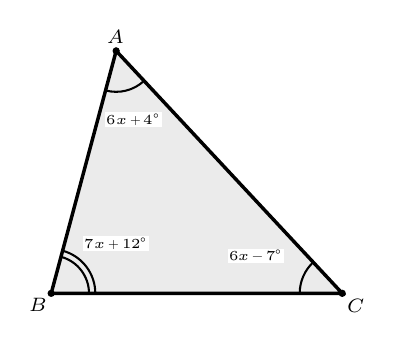
\begin{tikzpicture}[scale=0.88, every node/.style={font=\scriptsize, text=black}]
      % Exact 58-75-47 deg scalene triangle: B=(0,0), C=(4.20,0), A=(0.9375, 3.4987)
      \coordinate (B) at (0.0000, 0.0000);
      \coordinate (C) at (4.2000, 0.0000);
      \coordinate (A) at (0.9375, 3.4987);

      \fill[panelgray] (A) -- (B) -- (C) -- cycle;
      \draw[black, line width=1.25pt] (A) -- (B) -- (C) -- cycle;

      % Distinct angle arcs
      \pic[draw=black, line width=0.75pt, angle radius=5.2mm]{angle=B--A--C};
      \pic[draw=black, line width=0.75pt, angle radius=4.8mm]{angle=C--B--A};
      \pic[draw=black, line width=0.75pt, angle radius=5.6mm]{angle=C--B--A};
      \pic[draw=black, line width=0.75pt, angle radius=5.4mm]{angle=A--C--B};

      % Angle algebraic labels cleanly placed clear of lines
      \node[fill=white, inner sep=0.6pt, font=\tiny] at ($(A)+(-76:1.02)$) {$6x+4^\circ$};
      \node[fill=white, inner sep=0.6pt, font=\tiny] at ($(B)+(37.5:1.18)$) {$7x+12^\circ$};
      \node[fill=white, inner sep=0.6pt, font=\tiny] at ($(C)+(156.5:1.36)$) {$6x-7^\circ$};

      \fill[black] (A) circle (1.5pt) node[above=2pt, fill=white, inner sep=0.6pt] {$A$};
      \fill[black] (B) circle (1.5pt) node[below left=1.5pt, fill=white, inner sep=0.6pt] {$B$};
      \fill[black] (C) circle (1.5pt) node[below right=1.5pt, fill=white, inner sep=0.6pt] {$C$};
    \end{tikzpicture}
    \end{center}
    \begin{tcolorbox}[enhanced, sharp corners, colback=panelgray, colframe=black, boxrule=0.75pt, boxsep=1pt, top=3.5pt, bottom=3.5pt, left=5pt, right=5pt]
      \raggedright\fontsize{7.45pt}{10.4pt}\selectfont
      \textbf{ពិនិត្យក្រោយ (\en{EIA} ៣០ វិនាទី)៖}\\
      \textbf{១)} ហេតុអ្វី $\ang{B}=75^\circ$ ឈមនឹង $AC$ មិនមែន $AB$? ($B$ ជាកំពូល $\Rightarrow$ អក្សរទី ៣ បាត់គឺ $A, C$)\\
      \textbf{២)} ហេតុអ្វីមិនយក $75^\circ/47^\circ$ ធៀប $AC/AB$? ($x$ ជាអញ្ញាត; មុំមិនសមាមាត្រជ្រុង!)
    \end{tcolorbox}
  \end{minipage}\hfill
  \begin{minipage}[t]{10.20cm}
    \vspace{0pt}
    \begin{tcolorbox}[enhanced, sharp corners, colback=white, colframe=black, boxrule=0.85pt, boxsep=1pt, top=4pt, bottom=4pt, left=5pt, right=5pt]
      \raggedright\fontsize{7.75pt}{11.0pt}\selectfont
      \textbf{ជំហាន ១៖ ដោះស្រាយសមីការ $180^\circ$ (កែតម្រូវទំ.១៥៩ ដាក់ $^\circ$ លើ $9^\circ$)៖}\\[2pt]
      $\bullet$ $\ang{A}+\ang{B}+\ang{C}=180^\circ$ (\cnum{5}) $\Rightarrow (6x+4^\circ)+(7x+12^\circ)+(6x-7^\circ)=180^\circ$\\[2pt]
      $\bullet$ $19x + 9^\circ = 180^\circ \Rightarrow 19x = 180^\circ - \underline{\hspace{0.42cm}}^\circ = 171^\circ \Rightarrow x = \dfrac{171^\circ}{19} = \underline{\hspace{0.38cm}}^\circ$\\[2pt]
      $\bullet$ $\ang{A}=6(9^\circ)+4^\circ=\underline{\hspace{0.42cm}}^\circ$,\; $\ang{B}=7(9^\circ)+12^\circ=\underline{\hspace{0.42cm}}^\circ$,\; $\ang{C}=6(9^\circ)-7^\circ=\underline{\hspace{0.42cm}}^\circ$ \chkbox\ ($\Sigma=180^\circ$)
    \end{tcolorbox}
    \vspace{4pt}
    \begin{tcolorbox}[enhanced, sharp corners, colback=panelgray, colframe=black, boxrule=0.85pt, boxsep=1pt, top=4pt, bottom=4pt, left=5pt, right=5pt]
      \raggedright\fontsize{7.65pt}{10.8pt}\selectfont
      \textbf{ជំហាន ២៖ តារាងក្បួនអក្សរទី ៣ បាត់ (\en{[tracing]} កំពូលមុំ $\to$ ជ្រុងឈម, \cnum{1})៖}\\[3pt]
      {\setlength{\tabcolsep}{3pt}\renewcommand{\arraystretch}{1.20}%
      \begin{tabular}{|L{2.75cm}|L{2.10cm}|L{3.95cm}|}
        \hline
        \cellcolor{headgray}\textbf{មុំតាមលំដាប់} & \cellcolor{headgray}\textbf{អក្សរកំពូលបាត់} & \cellcolor{headgray}\textbf{ជ្រុងឈម (\en{[tracing]})} \\ \hline
        ធំជាងគេ៖ $\ang{B} = \underline{\hspace{0.42cm}}^\circ$ & អត់មាន $B \to A, C$ & ឈមនឹងជ្រុង $\underline{\hspace{0.62cm}}$ (វែងជាងគេ) \\ \hline
        កណ្ដាល៖ $\ang{A} = \underline{\hspace{0.42cm}}^\circ$ & អត់មាន $A \to B, C$ & ឈមនឹងជ្រុង $\underline{\hspace{0.62cm}}$ (កណ្ដាល) \\ \hline
        តូចជាងគេ៖ $\ang{C} = \underline{\hspace{0.42cm}}^\circ$ & អត់មាន $C \to A, B$ & ឈមនឹងជ្រុង $\underline{\hspace{0.62cm}}$ (ខ្លីជាងគេ) \\ \hline
      \end{tabular}}\\[3.5pt]
      \textbf{សន្និដ្ឋាន (\cnum{3})៖} ព្រោះ $\ang{B} > \ang{A} > \ang{C} \Rightarrow$ ជ្រុងពីធំទៅតូចគឺ $\underline{\hspace{0.65cm}} > \underline{\hspace{0.65cm}} > \underline{\hspace{0.65cm}}$~។
    \end{tcolorbox}
    \vspace{3pt}
    \raggedright{\fontsize{6.85pt}{9.5pt}\selectfont
    \textbf{ធនាគារ \cnum{1}--\cnum{5}៖} \cnum{1} ស្ពានមុំ-ជ្រុងឈម \en{|} \cnum{2} ផ្ទាល់ ៣.១ \en{|} \cnum{3} ច្រាស ៣.១ \en{|} \cnum{4} ចំណុច $D$ \& មុំក្រៅ \en{|} \cnum{5} $180^\circ$ / ៣ ករណី / ស្ពានស្មើ\par}
  \end{minipage}
\end{tcolorbox}%
}

\vspace{2pt}
\eFourCardINEQ{ប័ណ្ណទី ១}

\vspace{8pt}
\noindent\scissors\ \dotfill\ \textbf{កាត់តាមស្នាមចុចចែកជា ២ ប័ណ្ណ (\en{Cut Along Dashed Line})} \dotfill\ \scissors
\vspace{8pt}

\eFourCardINEQ{ប័ណ្ណទី ២}

\clearpage

% ============================================================================
% ទំព័រទី ៣៖ E5 Evaluate — "តុផ្ទៀងផ្ទាត់អក្សរឈម និងស្ពានអង្កត់ស្មើ ៣ តួនាទី" (ប្រតិបត្តិ ទំ.១៥៩ + E1)
% ============================================================================
\pagebanner{សម្ភារៈទី ៣៖ «តុផ្ទៀងផ្ទាត់អក្សរឈម និងស្ពានអង្កត់ស្មើ ៣ តួនាទី» \enbf{--} ប្រតិបត្តិ \enbf{(E5 \& E1)}}{ទំព័រ ៣/៦ \en{-- E5 Evaluate} (កាត់ ២ សន្លឹក \scissors)}

\newcommand{\eFiveSheetINEQ}[1]{%
\begin{tcolorbox}[
  enhanced, sharp corners, colback=white, colframe=white,
  borderline={1.0pt}{0pt}{black, dashed},
  boxsep=1pt, top=2.5pt, bottom=2.5pt, left=4.5pt, right=4.5pt
]
  \begin{tcolorbox}[
    enhanced, sharp corners, colback=headgray, colframe=black,
    boxrule=0.8pt, boxsep=1pt, top=2pt, bottom=2pt, left=4.5pt, right=4.5pt, after skip=3pt
  ]
    \fontsize{7.2pt}{9.8pt}\selectfont
    \textbf{\scissors\ តុផ្ទៀងផ្ទាត់អក្សរឈម និងស្ពានអង្កត់ស្មើ ៣ តួនាទី (#1)} \hfill ក្រុម៖ $\underline{\hspace{2.2cm}}$\\[1pt]
    \textbf{ប្រតិបត្តិ (ទំ.១៥៩)៖} ក្នុងរូប គេឱ្យ $AB = AC = BD$ និង $\ang{ABC} < \ang{BAC}$ ។ បង្ហាញថា $BD < BC$ ។
  \end{tcolorbox}

  \renewcommand{\arraystretch}{1.04}
  {\centering\setlength{\tabcolsep}{3.5pt}%
  \begin{tabular}{|L{6.55cm}|L{5.85cm}|L{5.20cm}|}
    \hline
    \cellcolor{panelgray}\centering\arraybackslash\fontsize{7.2pt}{9.5pt}\selectfont\textbf{តួនាទី ១៖ អ្នកគូសដាន \en{[tracing]} \en{\& Pause-Ask!}}\newline {\fontsize{6.5pt}{8.6pt}\selectfont សម្គាល់ \tickslash\ លើ $AB{=}AC{=}BD$ និងដាន $\tri{ABC}$} &
    \cellcolor{panelgray}\centering\arraybackslash\fontsize{7.2pt}{9.5pt}\selectfont\textbf{តួនាទី ២៖ អ្នកផ្គូផ្គងស្ពាន (\cnum{1}, \cnum{3}, \cnum{5})}\newline {\fontsize{6.5pt}{8.6pt}\selectfont ទាញ $AC < BC$ ពី $\tri{ABC}$ រួចជំនួសស្ពាន $BD=AC$} &
    \cellcolor{panelgray}\centering\arraybackslash\fontsize{7.2pt}{9.5pt}\selectfont\textbf{តួនាទី ៣៖ អ្នកពិនិត្យសំអាង \cnum{1}--\cnum{5} \en{\&} បិទ \en{E1}}\newline {\fontsize{6.5pt}{8.6pt}\selectfont \en{Pause-Review!} \en{\&} សរុបមេរៀនដងស្ទូច \en{E1}} \\ \hline

    % --- Column 1: MANDATORY Exact Euclidean Obtuse 108 deg Figure (R=2.2 cm, 1:1) ---
    {\centering
    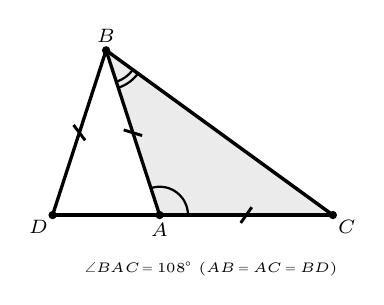
\begin{tikzpicture}[baseline={([yshift=-1ex]current bounding box.north)}, x=1cm, y=1cm, every node/.style={font=\scriptsize, text=black}]
      % Exact Obtuse Angle BAC = 108 deg, R = 2.2 cm:
      % A=(0,0), C=(2.2,0), B=(-0.6798, 2.0923), D=(-1.3597, 0)
      \coordinate (A) at (0.0000, 0.0000);
      \coordinate (C) at (2.2000, 0.0000);
      \coordinate (B) at (-0.6798, 2.0923);
      \coordinate (D) at (-1.3597, 0.0000);

      \fill[panelgray] (A) -- (B) -- (C) -- cycle;

      \draw[black, line width=1.2pt] (D) -- (A);
      \draw[black, line width=1.2pt, tkslash] (A) -- (C);
      \draw[black, line width=1.2pt, tkslash] (A) -- (B);
      \draw[black, line width=1.2pt, tkslash] (B) -- (D);
      \draw[black, line width=1.25pt] (B) -- (C);

      \pic[draw=black, line width=0.8pt, angle radius=3.6mm]{angle=C--A--B};
      \pic[draw=black, line width=0.8pt, angle radius=4.2mm]{angle=A--B--C};
      \pic[draw=black, line width=0.8pt, angle radius=5.0mm]{angle=A--B--C};

      \fill[black] (A) circle (1.5pt) node[below=2pt, fill=white, inner sep=0.6pt] {$A$};
      \fill[black] (C) circle (1.5pt) node[below right=1.5pt, fill=white, inner sep=0.6pt] {$C$};
      \fill[black] (B) circle (1.5pt) node[above=2pt, fill=white, inner sep=0.6pt] {$B$};
      \fill[black] (D) circle (1.5pt) node[below left=1.5pt, fill=white, inner sep=0.6pt] {$D$};

      \node[font=\tiny, fill=white, inner sep=0.4pt] at (0.42, -0.68) {ខ្នាតពិត $\ang{BAC}=108^\circ$ ($AB=AC=BD$)};
    \end{tikzpicture}\par\vspace{2pt}}
    \fontsize{7.0pt}{9.7pt}\selectfont
    \chkbox\ \textbf{\en{[tracing]}៖} អូសម្រាមដៃជុំវិញ $\tri{ABC}$ (ផ្ទៃប្រផេះ) និងគូស \tickslash\ លើ $AB=AC=BD$។\\[1.5pt]
    \chkbox\ \textbf{\en{Pause-Ask!}} ហេតុអ្វីមិនអាចប្រៀបធៀប $BD$ និង $BC$ ដោយមើលតែក្នុង $\tri{ABD}$ តែមួយ? (ខ្វះជ្រុង $BC$!)
    &
    % --- Column 2: Proof Bridge ---
    \fontsize{7.2pt}{10.2pt}\selectfont
    \textbf{ជំហាន ១៖ ក្នុងត្រីកោណតែមួយ ($\tri{ABC}$)}៖\par\vspace{1.5pt}
    $\bullet$ គេឱ្យ $\ang{ABC} < \ang{BAC}$\par\vspace{1.5pt}
    $\bullet$ $\ang{ABC}$ ឈមនឹងជ្រុង $\underline{\hspace{0.65cm}}$ (\cnum{1})\par\vspace{1.5pt}
    $\bullet$ $\ang{BAC}$ ឈមនឹងជ្រុង $\underline{\hspace{0.65cm}}$ (\cnum{1})\par\vspace{1.5pt}
    $\Rightarrow$ តាមទ្រឹស្ដីបទច្រាស (\cnum{3})៖\newline
    $\underline{\hspace{0.65cm}} < \underline{\hspace{0.65cm}}$\par\vspace{3pt}
    \textbf{ជំហាន ២៖ ស្ពានជំនួសអង្កត់ស្មើគ្នា}៖\par\vspace{1.5pt}
    $\bullet$ ដោយ $AB = AC = BD$ (\cnum{5})\par\vspace{1.5pt}
    $\bullet$ ជំនួស $AC$ ដោយ $\underline{\hspace{0.65cm}}$ $\Rightarrow \underline{\hspace{0.65cm}} < BC$ (ពិត!)\par\vspace{3pt}
    \begin{tcolorbox}[enhanced, sharp corners, colback=panelgray, colframe=black, boxrule=0.65pt, boxsep=1pt, top=2pt, bottom=2pt, left=4pt, right=4pt]
      \raggedright\fontsize{6.65pt}{9.2pt}\selectfont
      \textbf{ប្រើលេខសំអាង៖} \cnum{1} អក្សរឈម \en{|} \cnum{3} ច្រាស \en{|} \cnum{5} ស្ពានស្មើ
    \end{tcolorbox}
    &
    % --- Column 3: Pause-Review & E1 Closure ---
    \fontsize{7.05pt}{9.8pt}\selectfont
    \chkbox\ \textbf{\en{Pause-Review!}} ផ្ទៀង៖\newline
    ១) ហេតុអ្វី $\ang{BAC}=108^\circ > 90^\circ$? (បើមុំស្រួច $BD$ មិនអាចស្មើ $AB$ តាមបាតអ៊ីសូសែល $72^\circ$ បានទេ!)\newline
    ២) មានលេខ \cnum{1}, \cnum{3}, \cnum{5} គ្រប់ និងគ្មានអក្សរឈមច្រឡំ!\par\vspace{3pt}
    \begin{tcolorbox}[enhanced, sharp corners, colback=panelgray, colframe=black, boxrule=0.7pt, boxsep=1pt, top=2.5pt, bottom=2.5pt, left=4pt, right=4pt]
      \raggedright\fontsize{6.75pt}{9.4pt}\selectfont
      \textbf{បិទបេសកកម្ម \en{E1} (ដងស្ទូចទ្វារទឹក)៖}\\
      ក្នុងដងស្ទូច $4\unit{m}$ និង $7\unit{m}$៖ មុំហ៊ីងបើកកាន់តែធំ ខ្សែកាបឈមត្រូវវែងតាមលំដាប់ (\cnum{2}, \cnum{3}) តែមុំគុណ ២ \textbf{មិន}នាំឱ្យខ្សែកាបគុណ ២ ឡើយ!
    \end{tcolorbox}
    \\ \hline
  \end{tabular}\par}
\end{tcolorbox}%
}

\eFiveSheetINEQ{សន្លឹកទី ១}

\vspace{3.5pt}
\noindent\scissors\ \dotfill\ \textbf{កាត់តាមស្នាមចុចចែកជា ២ សន្លឹក (\en{Cut Along Dashed Line})} \dotfill\ \scissors
\vspace{3.5pt}

\eFiveSheetINEQ{សន្លឹកទី ២}

\clearpage

% ============================================================================
% ទំព័រទី ៤៖ ផ្ទាំងសំអាងគោល ៣.១ — វិសមភាពចំពោះជ្រុងនិងមុំនៃត្រីកោណមួយ & ធនាគារ ①–⑤
% ============================================================================
\begin{tcolorbox}[
  enhanced, sharp corners, colback=white, colframe=black,
  boxrule=1.5pt, borderline={0.6pt}{2.2pt}{black},
  boxsep=1pt, top=9pt, bottom=9pt, left=6.5pt, right=6.5pt
]
  \begin{center}
    {\fontsize{8.0pt}{11.0pt}\selectfont មន្ទីរអប់រំ យុវជន និងកីឡា ខេត្តកំពង់ធំ \en{|} ការិយាល័យអប់រំ យុវជន និងកីឡា ស្រុកកំពង់ស្វាយ \en{|} អនុវិទ្យាល័យព្រះក្រសាំង}\\[2.5pt]
    {\muol\fontsize{11.6pt}{16.8pt}\selectfont ផ្ទាំងសំអាងគោល ៣\enbf{.}១៖ វិសមភាពចំពោះជ្រុងនិងមុំនៃត្រីកោណមួយ \enbf{(}\cnum{1}\enbf{--}\cnum{5}\enbf{)}}\\[2.5pt]
    {\fontsize{7.4pt}{10.5pt}\selectfont គណិតវិទ្យា ថ្នាក់ទី៨ \en{--} មេរៀនទី១២ (ទំ.១៥៨\en{--}១៥៩) \en{|} គ្រូបង្រៀន៖ ហុក ប៊ុនថែន \en{|} ថ្ងៃព្រហស្បតិ៍ ៩រោច ខែកត្តិក ឆ្នាំមមី អដ្ឋស័ក ព.ស. ២៥៧០ (ថ្ងៃព្រហស្បតិ៍ ទី៣ ខែធ្នូ ឆ្នាំ២០២៦)}\\[4pt]
    \khmflourish
  \end{center}
  \vspace{8pt}

  % --- ផ្នែកទី ១៖ សម្រាយផ្ទាល់ ឧទាហរណ៍ ទំ.១៥៨ (ឆ្វេង) & ប្រអប់ទ្រឹស្ដីបទ កែទំ.១៥៨ + ៣ ករណី (ស្ដាំ) ---
  \noindent
  \begin{minipage}[t]{8.90cm}
    \begin{tcolorbox}[enhanced, sharp corners, colback=white, colframe=black, boxrule=0.95pt, boxsep=1pt, equal height group=posterTopINEQ, top=7pt, bottom=7pt, left=5.5pt, right=5.5pt]
      \textbf{\fontsize{8.2pt}{11.4pt}\selectfont សម្រាយផ្ទាល់ (ឧទាហរណ៍ ទំ.១៥៨)៖ $AC > AB \Rightarrow \ang{B} > \ang{C}$}\\[5pt]
      \begin{minipage}[c]{3.65cm}
        \centering
        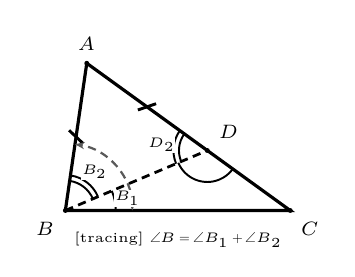
\begin{tikzpicture}[scale=0.68, every node/.style={font=\scriptsize, text=black}]
          % B=(0,0), C=(4.20,0), A=(0.40,2.75), D=(2.6513,1.1208)
          \coordinate (B) at (0.00, 0.00);
          \coordinate (C) at (4.20, 0.00);
          \coordinate (A) at (0.40, 2.75);
          \coordinate (D) at (2.6513, 1.1208);

          \draw[black, line width=1.15pt, tkslash] (A) -- (B);
          \draw[black, line width=1.15pt, tkslash] (A) -- (D);
          \draw[black, line width=1.15pt] (D) -- (C) -- (B);
          \draw[black, densely dashed, line width=1.0pt] (B) -- (D);

          % [tracing] arc along B = B1 + B2
          \draw[darkline, densely dashed, line width=0.8pt, {Stealth[length=1.2mm]}-{Stealth[length=1.2mm]}]
            ($(B)+(0:1.25)$) arc (0:81.7:1.25);

          % Double arcs (2) at B2 & D2; Single arcs (1) at B1 & D1
          \pic[draw=black, line width=0.7pt, angle radius=3.8mm]{angle=D--B--A};
          \pic[draw=black, line width=0.7pt, angle radius=4.5mm]{angle=D--B--A};
          \pic[draw=black, line width=0.7pt, angle radius=6.4mm]{angle=C--B--D};
          \pic[draw=black, line width=0.7pt, angle radius=3.6mm]{angle=A--D--B};
          \pic[draw=black, line width=0.7pt, angle radius=4.3mm]{angle=A--D--B};
          \pic[draw=black, line width=0.7pt, angle radius=4.0mm]{angle=B--D--C};

          \node[font=\tiny, fill=white, inner sep=0.4pt] at ($(B)+(53:0.90)$) {$B_2$};
          \node[font=\tiny, fill=white, inner sep=0.4pt] at ($(B)+(11:1.18)$) {$B_1$};
          \node[font=\tiny, fill=white, inner sep=0.4pt] at ($(D)+(173:0.86)$) {$D_2$};

          \fill[black] (A) circle (1.3pt) node[above=1pt] {$A$};
          \fill[black] (B) circle (1.3pt) node[below left=1pt] {$B$};
          \fill[black] (C) circle (1.3pt) node[below right=1pt] {$C$};
          \fill[black] (D) circle (1.3pt) node[above right=1pt] {$D$};
          \node[font=\tiny, fill=white, inner sep=0.4pt] at (2.10, -0.55) {\en{[tracing]} $\ang{B}=\ang{B_1}+\ang{B_2}$};
        \end{tikzpicture}
      \end{minipage}\hfill
      \begin{minipage}[c]{4.65cm}
        \raggedright\fontsize{7.55pt}{11.2pt}\selectfont
        \textbf{១.} ដៅ $D\in AC$: $AD=AB<AC \Rightarrow D$ នៅ\textbf{ចន្លោះ} $A, C$ (\cnum{4})។\\[3pt]
        \textbf{២.} $\tri{ABD}$ សមបាទ $\Rightarrow \ang{B_2}=\ang{D_2}$។\\[3pt]
        \textbf{៣.} មុំក្រៅ $\tri{BCD}$: $\ang{D_2}=\ang{B_1}+\ang{C} > \ang{C}$ (\cnum{4})។\\[3pt]
        \textbf{៤.} $\ang{B}=\ang{B_1}+\ang{B_2} > \ang{B_2} = \ang{D_2} > \ang{C}$ $\Rightarrow \ang{B} > \ang{C}$~។
      \end{minipage}
    \end{tcolorbox}
  \end{minipage}\hfill
  \begin{minipage}[t]{8.80cm}
    \begin{tcolorbox}[enhanced, sharp corners, colback=panelgray, colframe=black, boxrule=0.95pt, boxsep=1pt, equal height group=posterTopINEQ, top=7pt, bottom=7pt, left=5.5pt, right=5.5pt]
      \raggedright\fontsize{7.65pt}{10.8pt}\selectfont
      \textbf{ទ្រឹស្ដីបទ ៣.១ (កែតម្រូវទំ.១៥៨) \& សម្រាយច្រាស ៣ ករណី៖}\\[2pt]
      $\bullet$ \textbf{ផ្ទាល់៖} បើជ្រុងពីរមិនប៉ុនគ្នា មុំដែលឈមនឹងជ្រុងទាំងពីរនេះក៏មិនប៉ុនគ្នាដែរ ហើយមុំដែលឈមនឹងជ្រុងធំជាង ជាមុំធំជាង\textbf{។}\\[2pt]
      $\bullet$ \textbf{ច្រាស៖} ច្រាសមកវិញ បើមុំពីរមិនប៉ុនគ្នា ជ្រុងដែលឈមនឹងមុំទាំងពីរនេះ\textbf{ក៏មិនប៉ុនគ្នាដែរ} ហើយជ្រុងដែលឈមនឹងមុំធំជាង ជាជ្រុងធំជាង។ \textit{(កែ «ក៏មានប៉ុនគ្នាដែរ» $\to$ «ក៏មិនប៉ុនគ្នាដែរ»!)}\\[4pt]
      % Converse 3-case Trichotomy mini-diagram
      \centering
      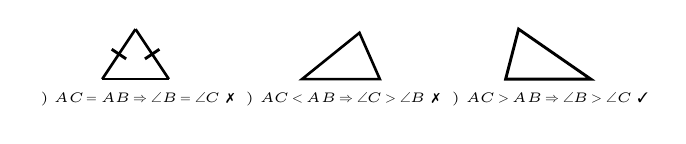
\begin{tikzpicture}[scale=0.47, every node/.style={font=\tiny, text=black}]
        \begin{scope}[shift={(0,0)}]
          \draw[black, line width=0.95pt, tk1] (0.9,1.35)--(0,0);
          \draw[black, line width=0.95pt, tk1] (0.9,1.35)--(1.8,0);
          \draw[black, line width=0.95pt] (0,0)--(1.8,0);
          \node at (0.9,-0.55) {១) $AC=AB\Rightarrow\ang{B}=\ang{C}$ \ding{55}};
        \end{scope}
        \begin{scope}[shift={(5.4,0)}]
          \draw[black, line width=0.95pt] (0,0)--(2.1,0)--(1.55,1.25)--cycle;
          \node at (1.05,-0.55) {២) $AC<AB\Rightarrow\ang{C}>\ang{B}$ \ding{55}};
        \end{scope}
        \begin{scope}[shift={(10.9,0)}]
          \draw[black, line width=1.05pt] (0,0)--(2.3,0)--(0.35,1.35)--cycle;
          \node at (1.15,-0.55) {៣) $AC>AB\Rightarrow\ang{B}>\ang{C}$ \ding{51}};
        \end{scope}
      \end{tikzpicture}
    \end{tcolorbox}
  \end{minipage}

  \vspace{8pt}

  % --- ផ្នែកទី ២៖ តារាងធនាគារអំណះអំណាង ①–⑤ (ពាក្យ-ទល់-ពាក្យ ១០០% នឹង LS_Plan) ---
  \fontsize{8.0pt}{11.6pt}\selectfont
  \renewcommand{\arraystretch}{1.42}
  \begin{tabular}{|C{0.72cm}|L{4.35cm}|L{6.55cm}|C{4.55cm}|}
    \hline
    \cellcolor{headgray}\textbf{លេខ} &
    \cellcolor{headgray}\centering\arraybackslash\textbf{ឈ្មោះអំណះអំណាង} &
    \cellcolor{headgray}\centering\arraybackslash\textbf{និមិត្តសញ្ញា និងរបៀបប្រើ} &
    \cellcolor{headgray}\centering\arraybackslash\textbf{រូបសម្គាល់ ស-ខ្មៅ} \\ \hline

    \cnum{1} &
    \textbf{ស្ពានមុំឈម–ជ្រុងឈម} &
    ក្បួនអក្សរទី ៣ ដែលបាត់ក្នុងត្រីកោណតែមួយ ($\tri{ABC}$៖ $\ang{A}\leftrightarrow BC$, $\ang{B}\leftrightarrow AC$, $\ang{C}\leftrightarrow AB$)~។ &
    \raisebox{-0.35\height}{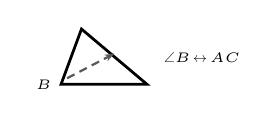
\begin{tikzpicture}[scale=0.52, every node/.style={font=\tiny, text=black}]
      \coordinate (b) at (0,0); \coordinate (c) at (2.1,0); \coordinate (a) at (0.5,1.35);
      \draw[black, line width=1.0pt] (a)--(b)--(c)--cycle;
      \draw[darkline, densely dashed, line width=0.8pt, -{Stealth[length=1.2mm]}] (0.15,0.15)--(1.3,0.75);
      \node[left=0pt] at (b) {$B$}; \node[right=2pt] at (2.15,0.65) {$\ang{B}\leftrightarrow AC$};
    \end{tikzpicture}} \\ \hline

    \cnum{2} &
    \textbf{ទ្រឹស្ដីបទផ្ទាល់ ៣.១} &
    ក្នុងត្រីកោណមួយ ជ្រុងធំជាង $\Rightarrow$ មុំឈមធំជាង ($AC>AB \Rightarrow \ang{B}>\ang{C}$)~។ &
    \raisebox{-0.35\height}{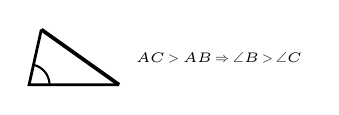
\begin{tikzpicture}[scale=0.52, every node/.style={font=\tiny, text=black}]
      \coordinate (b) at (0,0); \coordinate (c) at (2.2,0); \coordinate (a) at (0.3,1.35);
      \draw[black, line width=1.0pt] (a)--(b)--(c);
      \draw[black, line width=1.35pt] (a)--(c);
      \pic[draw=black, line width=0.75pt, angle radius=2.6mm]{angle=c--b--a};
      \node[right=2pt] at (2.25,0.65) {$AC>AB\Rightarrow\ang{B}>\ang{C}$};
    \end{tikzpicture}} \\ \hline

    \cnum{3} &
    \textbf{ទ្រឹស្ដីបទច្រាស ៣.១} &
    ក្នុងត្រីកោណមួយ មុំធំជាង $\Rightarrow$ ជ្រុងឈមធំជាង — \textbf{ក៏មិនប៉ុនគ្នាដែរ} ($\ang{B}>\ang{C}\Rightarrow AC>AB$)~។ &
    \raisebox{-0.35\height}{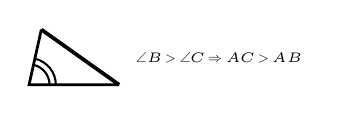
\begin{tikzpicture}[scale=0.52, every node/.style={font=\tiny, text=black}]
      \coordinate (b) at (0,0); \coordinate (c) at (2.2,0); \coordinate (a) at (0.3,1.35);
      \draw[black, line width=1.0pt] (a)--(b)--(c);
      \draw[black, line width=1.35pt] (a)--(c);
      \pic[draw=black, line width=0.75pt, angle radius=2.6mm]{angle=c--b--a};
      \pic[draw=black, line width=0.75pt, angle radius=3.4mm]{angle=c--b--a};
      \node[right=2pt] at (2.25,0.65) {$\ang{B}>\ang{C}\Rightarrow AC>AB$};
    \end{tikzpicture}} \\ \hline

    \cnum{4} &
    \textbf{សំណង់ចំណុចជំនួយ និងមុំក្រៅត្រីកោណ} &
    $AD=AB<AC \Rightarrow D$ ចន្លោះ $A,C$ និង $\ang{\text{ក្រៅ}} > \ang{\text{ក្នុងមិនជាប់}}$ ($\ang{D_2}=\ang{B_1}+\ang{C}>\ang{C}$)~។ &
    \raisebox{-0.35\height}{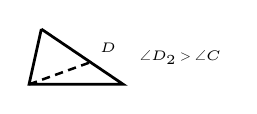
\begin{tikzpicture}[scale=0.52, every node/.style={font=\tiny, text=black}]
      \coordinate (b) at (0,0); \coordinate (c) at (2.3,0); \coordinate (a) at (0.3,1.35); \coordinate (d) at (1.5,0.54);
      \draw[black, line width=1.0pt] (a)--(b)--(c)--(a); \draw[black, densely dashed, line width=0.9pt] (b)--(d);
      \node[above right=0pt] at (d) {$D$}; \node[right=2pt] at (2.35,0.65) {$\ang{D_2}>\ang{C}$};
    \end{tikzpicture}} \\ \hline

    \cnum{5} &
    \textbf{ផលបូក $180^\circ$ / ៣ ករណី / ស្ពានស្មើ} &
    $\ang{A}+\ang{B}+\ang{C}=180^\circ$; បីករណី ($=, <, >$) និងស្ពានជំនួសអង្កត់ស្មើគ្នា ($BD=AC$)~។ &
    \raisebox{-0.35\height}{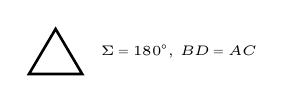
\begin{tikzpicture}[scale=0.52, every node/.style={font=\tiny, text=black}]
      \draw[black, line width=0.95pt] (0,0)--(1.3,0)--(0.65,1.1)--cycle;
      \node[right=2pt] at (1.4,0.55) {$\Sigma=180^\circ$, $BD=AC$};
    \end{tikzpicture}} \\ \hline
  \end{tabular}

  \vspace{8pt}

  % --- ផ្នែកទី ៣៖ ក្បួនអក្សរទី ៣ បាត់ (ឆ្វេង) & អន្ទាក់ផលធៀបលីនេអ៊ែរ (ស្ដាំ) ---
  \noindent
  \begin{minipage}[t]{8.85cm}
    \begin{tcolorbox}[
      enhanced, sharp corners, colback=white, colframe=black,
      boxrule=1.05pt, boxsep=1pt, equal height group=posterBotINEQ,
      top=7pt, bottom=7pt, left=5.5pt, right=5.5pt,
      title={\textbf{ក្បួនអក្សរទី ៣ ដែលបាត់ (\en{Missing-Letter Rule})}},
      colbacktitle=headgray, coltitle=black, fonttitle=\fontsize{8.2pt}{11.2pt}\selectfont
    ]
      \centering
      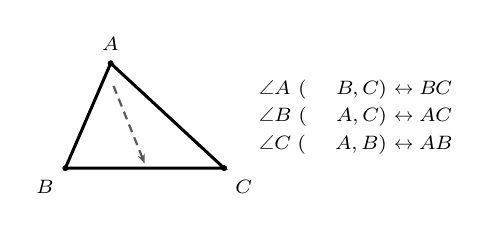
\begin{tikzpicture}[scale=0.72, every node/.style={font=\scriptsize, text=black}]
        \coordinate (A) at (0.8, 1.85); \coordinate (B) at (0, 0); \coordinate (C) at (2.8, 0);
        \draw[black, line width=1.1pt] (A)--(B)--(C)--cycle;
        \draw[darkline, densely dashed, line width=0.8pt, -{Stealth[length=1.2mm]}] (0.85,1.45)--(1.40,0.08);
        \fill[black] (A) circle (1.5pt) node[above=1pt] {$A$};
        \fill[black] (B) circle (1.5pt) node[below left=1pt] {$B$};
        \fill[black] (C) circle (1.5pt) node[below right=1pt] {$C$};
        \node[right=5pt, align=left, font=\scriptsize] at (3.0, 0.90)
          {$\ang{A}$ (បាត់ $B,C$) $\leftrightarrow BC$\\[2pt]
           $\ang{B}$ (បាត់ $A,C$) $\leftrightarrow AC$\\[2pt]
           $\ang{C}$ (បាត់ $A,B$) $\leftrightarrow AB$};
      \end{tikzpicture}
      \par\vspace{5pt}\fontsize{7.7pt}{11.2pt}\selectfont
      $\bullet$ \textbf{ច្បាប់ដែក៖} ប្រើបានតែក្នុង\textbf{ត្រីកោណតែមួយ} ($\tri{ABC}$) — ហាមឆ្លងត្រីកោណផ្សេងដែលគ្មានស្ពានស្មើភ្ជាប់!
    \end{tcolorbox}
  \end{minipage}\hfill
  \begin{minipage}[t]{8.85cm}
    \begin{tcolorbox}[
      enhanced, sharp corners, colback=white, colframe=black,
      boxrule=1.05pt, boxsep=1pt, equal height group=posterBotINEQ,
      top=7pt, bottom=7pt, left=5.5pt, right=5.5pt,
      title={\ding{55}\ \textbf{ព្រមាន៖ អន្ទាក់ផលធៀបលីនេអ៊ែរ ($\ang{B}=2\ang{C}\not\Rightarrow AC=2AB$)}},
      colbacktitle=midgray, coltitle=black, fonttitle=\fontsize{8.2pt}{11.2pt}\selectfont
    ]
      \centering
      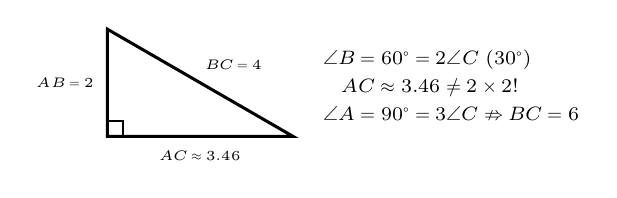
\begin{tikzpicture}[scale=0.68, every node/.style={font=\tiny, text=black}]
        \coordinate (A) at (0,0); \coordinate (C) at (3.464,0); \coordinate (B) at (0,2.0);
        \draw[black, line width=1.1pt] (A)--(C)--(B)--cycle;
        \pic[draw=black, line width=0.7pt, angle radius=2.0mm]{right angle=C--A--B};
        \node[below=1.5pt] at (1.73, 0) {$AC\approx 3.46$};
        \node[left=1.5pt] at (0, 1.0) {$AB=2$};
        \node[above right=0pt] at (1.65, 1.05) {$BC=4$};
        \node[right=4pt, align=left, font=\scriptsize] at (3.65, 0.95)
          {$\ang{B}=60^\circ = 2\ang{C}$ ($30^\circ$)\\[2pt]
           តែ $AC\approx 3.46 \neq 2\times 2$!\\[2pt]
           $\ang{A}=90^\circ = 3\ang{C} \not\Rightarrow BC=6$};
      \end{tikzpicture}
      \par\vspace{5pt}\fontsize{7.7pt}{11.2pt}\selectfont
      \textbf{ចងចាំ៖} រក្សាតែ \textbf{លំដាប់ ($<, >$)} មិនមែនផលធៀបគុណ ($\times 2, \times 3$) ទេ!
    \end{tcolorbox}
  \end{minipage}
  \par\vspace{7pt}
  \begin{tcolorbox}[enhanced, sharp corners, colback=panelgray, colframe=black, boxrule=0.75pt, boxsep=1pt, top=4pt, bottom=4pt, left=6pt, right=6pt]
    \centering\fontsize{7.7pt}{11.0pt}\selectfont
    \textbf{គោលការណ៍ប្រើផ្ទាំងសំអាងក្នុងថ្នាក់ (\en{E3--E5})៖} រាល់ជំហានបកស្រាយក្នុង \textbf{លំហាត់គំរូ (ទំ.១៥៨--១៥៩)}, \textbf{ប្រតិបត្តិ (ទំ.១៥៩)} និង \textbf{លំហាត់ទី ១៣--១៥ (ទំ.១៦៦)} ត្រូវចុះលេខសំអាង \cnum{1}--\cnum{5} ភ្ជាប់ជានិច្ច!
  \end{tcolorbox}
\end{tcolorbox}

\clearpage

% ============================================================================
% ទំព័រទី ៥៖ កាតវិនិច្ឆ័យរហ័ស "កាត A–D" & សំបុត្រចេញ ៣ សំណួរ — E5 Evaluate
% ============================================================================
\pagebanner{សម្ភារៈទី ៥៖ កាតវិនិច្ឆ័យរហ័ស «កាត \enbf{A--D}» \enbf{\&} សំបុត្រចេញរហ័ស \enbf{E5}}{ទំព័រ ៥/៦ \en{-- E5 Evaluate}}

{\fontsize{8.3pt}{11.6pt}\selectfont
\textbf{វិធីលេងក្នុងថ្នាក់៖} គ្រូលើកកាតម្ដងមួយ $\rightarrow$ សិស្សផ្ទៀងលក្ខខណ្ឌកំពូលឈម / ផលធៀប / ត្រីកោណតែមួយ $\rightarrow$ លើក \textbf{មេដៃឡើង (ពិត \ding{51})} ឬ \textbf{ខ្វែងដៃ (ខុស/អន្ទាក់ \ding{55})} + ម្រាម \en{1--3}។}

\vspace{5pt}

% --- ជួរទី ១៖ កាត A & កាត B ---
\noindent
\begin{tcolorbox}[
  enhanced, sharp corners, colback=white, colframe=white,
  borderline={1.0pt}{0pt}{black, dashed},
  width=9.25cm, equal height group=ineqfoilrow1, nobeforeafter,
  boxsep=1pt, top=5pt, bottom=5pt, left=6pt, right=6pt
]
  \noindent\colorbox{black}{\textcolor{white}{\Large\textbf{\en{ A }}}}\hspace{0.22cm}{\fontsize{8.9pt}{12.0pt}\selectfont\textbf{កាត \en{A} ៖ លំដាប់មុំ $\to$ លំដាប់ជ្រុង ($\tri{PQR}$)}}\par\vspace{2pt}
  \begin{center}
  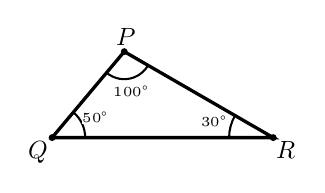
\begin{tikzpicture}[scale=0.78, every node/.style={font=\small, text=black}]
    % P=100, Q=50, R=30: Q=(0,0), R=(3.60,0), P=(1.1749,1.4002)
    \coordinate (Q) at (0, 0);
    \coordinate (R) at (3.60, 0);
    \coordinate (P) at (1.1749, 1.4002);
    \draw[black, line width=1.2pt] (P) -- (Q) -- (R) -- cycle;
    \pic[draw=black, line width=0.75pt, angle radius=3.5mm]{angle=Q--P--R};
    \pic[draw=black, line width=0.75pt, angle radius=4.2mm]{angle=R--Q--P};
    \pic[draw=black, line width=0.75pt, angle radius=5.6mm]{angle=P--R--Q};
    \node[fill=white, inner sep=0.4pt, font=\tiny] at ($(P)+(-80:0.65)$) {$100^\circ$};
    \node[fill=white, inner sep=0.4pt, font=\tiny] at ($(Q)+(25:0.78)$) {$50^\circ$};
    \node[fill=white, inner sep=0.4pt, font=\tiny] at ($(R)+(165:1.00)$) {$30^\circ$};
    \fill[black] (P) circle (1.6pt) node[above=1.5pt, fill=white, inner sep=0.4pt] {$P$};
    \fill[black] (Q) circle (1.6pt) node[below left=1pt, fill=white, inner sep=0.4pt] {$Q$};
    \fill[black] (R) circle (1.6pt) node[below right=1pt, fill=white, inner sep=0.4pt] {$R$};
  \end{tikzpicture}
  \end{center}
  {\centering\fontsize{7.9pt}{10.8pt}\selectfont ក្នុង $\tri{PQR}$៖ $\ang{P}=100^\circ, \ang{Q}=50^\circ, \ang{R}=30^\circ$។\newline គេទាញថា $QR > PR > PQ$។\par}
  \vfill
  \begin{tcolorbox}[enhanced, sharp corners, colback=panelgray, colframe=black, boxrule=0.8pt, boxsep=1pt, top=3.5pt, bottom=3.5pt, left=4pt, right=4pt]
    \centering\fontsize{8.7pt}{11.8pt}\selectfont
    \textbf{សំណួរ៖} ត្រឹមត្រូវឬទេ? \quad \chkbox~ពិត (\ding{51}) \quad \chkbox~ខុស (\ding{55})
  \end{tcolorbox}
\end{tcolorbox}%
\hfill
\begin{tcolorbox}[
  enhanced, sharp corners, colback=white, colframe=white,
  borderline={1.0pt}{0pt}{black, dashed},
  width=9.25cm, equal height group=ineqfoilrow1, nobeforeafter,
  boxsep=1pt, top=5pt, bottom=5pt, left=6pt, right=6pt
]
  \noindent\colorbox{black}{\textcolor{white}{\Large\textbf{\en{ B }}}}\hspace{0.22cm}{\fontsize{8.9pt}{12.0pt}\selectfont\textbf{កាត \en{B} ៖ អន្ទាក់កំពូលឈម ($5, 8, 6\unit{cm}$)}}\par\vspace{2pt}
  \begin{center}
  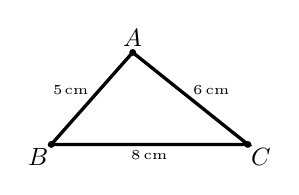
\begin{tikzpicture}[scale=0.78, every node/.style={font=\small, text=black}]
    % AB=5, BC=8, AC=6 (*0.4): B=(0,0), C=(3.20,0), A=(1.3250,1.4981)
    \coordinate (B) at (0, 0);
    \coordinate (C) at (3.20, 0);
    \coordinate (A) at (1.3250, 1.4981);
    \draw[black, line width=1.2pt] (A) -- (B) -- (C) -- cycle;
    \fill[black] (A) circle (1.6pt) node[above=1.5pt, fill=white, inner sep=0.4pt] {$A$};
    \fill[black] (B) circle (1.6pt) node[below left=1pt, fill=white, inner sep=0.4pt] {$B$};
    \fill[black] (C) circle (1.6pt) node[below right=1pt, fill=white, inner sep=0.4pt] {$C$};
    \node[above left=1pt, fill=white, inner sep=0.4pt, font=\tiny] at ($(A)!0.50!(B)$) {$5\unit{cm}$};
    \node[below=1.5pt, fill=white, inner sep=0.4pt, font=\tiny] at ($(B)!0.50!(C)$) {$8\unit{cm}$};
    \node[above right=1pt, fill=white, inner sep=0.4pt, font=\tiny] at ($(A)!0.50!(C)$) {$6\unit{cm}$};
  \end{tikzpicture}
  \end{center}
  {\centering\fontsize{7.9pt}{10.8pt}\selectfont ក្នុង $\tri{ABC}$៖ $AB=5\unit{cm}, BC=8\unit{cm}, AC=6\unit{cm}$។\newline គេអះអាងថា $\ang{B}$ ជាមុំធំជាងគេ (ព្រោះ $BC$ មាន $B$)! \par}
  \vfill
  \begin{tcolorbox}[enhanced, sharp corners, colback=panelgray, colframe=black, boxrule=0.8pt, boxsep=1pt, top=3.5pt, bottom=3.5pt, left=4pt, right=4pt]
    \centering\fontsize{8.7pt}{11.8pt}\selectfont
    \textbf{សំណួរ៖} ត្រឹមត្រូវឬទេ? \quad \chkbox~ពិត (\ding{51}) \quad \chkbox~ខុស (\ding{55})
  \end{tcolorbox}
\end{tcolorbox}

\vspace{6pt}

% --- ជួរទី ២៖ កាត C & កាត D ---
\noindent
\begin{tcolorbox}[
  enhanced, sharp corners, colback=white, colframe=white,
  borderline={1.0pt}{0pt}{black, dashed},
  width=9.25cm, equal height group=ineqfoilrow2, nobeforeafter,
  boxsep=1pt, top=5pt, bottom=5pt, left=6pt, right=6pt
]
  \noindent\colorbox{black}{\textcolor{white}{\Large\textbf{\en{ C }}}}\hspace{0.22cm}{\fontsize{8.9pt}{12.0pt}\selectfont\textbf{កាត \en{C} ៖ អន្ទាក់ផលធៀបគុណ ២ ($\tri{MNP}$)}}\par\vspace{2pt}
  \begin{center}
  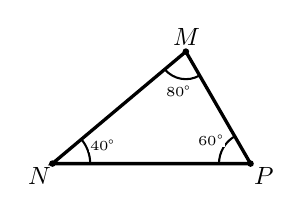
\begin{tikzpicture}[scale=0.74, every node/.style={font=\small, text=black}]
    % M=80, N=40, P=60: N=(0,0), P=(3.40,0), M=(2.2904,1.9219)
    \coordinate (N) at (0, 0);
    \coordinate (P) at (3.40, 0);
    \coordinate (M) at (2.2904, 1.9219);
    \draw[black, line width=1.2pt] (M) -- (N) -- (P) -- cycle;
    \pic[draw=black, line width=0.75pt, angle radius=3.5mm]{angle=N--M--P};
    \pic[draw=black, line width=0.75pt, angle radius=4.8mm]{angle=P--N--M};
    \pic[draw=black, line width=0.75pt, angle radius=4.0mm]{angle=M--P--N};
    \node[fill=white, inner sep=0.4pt, font=\tiny] at ($(M)+(-100:0.70)$) {$80^\circ$};
    \node[fill=white, inner sep=0.4pt, font=\tiny] at ($(N)+(20:0.92)$) {$40^\circ$};
    \node[fill=white, inner sep=0.4pt, font=\tiny] at ($(P)+(150:0.78)$) {$60^\circ$};
    \fill[black] (M) circle (1.6pt) node[above=1.5pt, fill=white, inner sep=0.4pt] {$M$};
    \fill[black] (N) circle (1.6pt) node[below left=1pt, fill=white, inner sep=0.4pt] {$N$};
    \fill[black] (P) circle (1.6pt) node[below right=1pt, fill=white, inner sep=0.4pt] {$P$};
  \end{tikzpicture}
  \end{center}
  {\centering\fontsize{7.9pt}{10.8pt}\selectfont ក្នុង $\tri{MNP}$៖ $\ang{M}=80^\circ, \ang{N}=40^\circ, \ang{P}=60^\circ$។\newline គេអះអាងថា ព្រោះ $\ang{M}=2\ang{N}$ នោះ $NP = 2MP$។\par}
  \vfill
  \begin{tcolorbox}[enhanced, sharp corners, colback=panelgray, colframe=black, boxrule=0.8pt, boxsep=1pt, top=3.5pt, bottom=3.5pt, left=4pt, right=4pt]
    \centering\fontsize{8.7pt}{11.8pt}\selectfont
    \textbf{សំណួរ៖} ត្រឹមត្រូវឬទេ? \quad \chkbox~ពិត (\ding{51}) \quad \chkbox~ខុស (\ding{55})
  \end{tcolorbox}
\end{tcolorbox}%
\hfill
\begin{tcolorbox}[
  enhanced, sharp corners, colback=white, colframe=white,
  borderline={1.0pt}{0pt}{black, dashed},
  width=9.25cm, equal height group=ineqfoilrow2, nobeforeafter,
  boxsep=1pt, top=5pt, bottom=5pt, left=6pt, right=6pt
]
  \noindent\colorbox{black}{\textcolor{white}{\Large\textbf{\en{ D }}}}\hspace{0.22cm}{\fontsize{8.9pt}{12.0pt}\selectfont\textbf{កាត \en{D} ៖ អន្ទាក់ត្រីកោណ ២ ដាច់ពីគ្នា}}\par\vspace{2pt}
  \begin{center}
  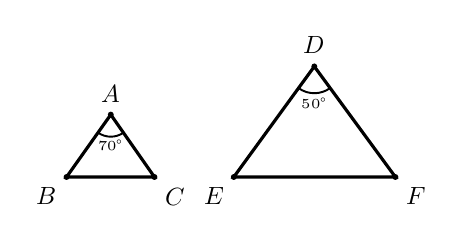
\begin{tikzpicture}[scale=0.72, every node/.style={font=\small, text=black}]
    % Small ABC (A=70 deg) vs Large DEF (D=50 deg) with wide gap between C and E
    \begin{scope}[shift={(0,0)}]
      \coordinate (B) at (0,0); \coordinate (C) at (1.55,0); \coordinate (A) at (0.78,1.10);
      \draw[black, line width=1.15pt] (A)--(B)--(C)--cycle;
      \pic[draw=black, line width=0.7pt, angle radius=2.8mm]{angle=B--A--C};
      \node[fill=white, inner sep=0.3pt, font=\tiny] at ($(A)+(-90:0.54)$) {$70^\circ$};
      \fill[black] (A) circle (1.5pt) node[above=1pt] {$A$};
      \fill[black] (B) circle (1.5pt) node[below left=0.5pt] {$B$};
      \fill[black] (C) circle (1.5pt) node[below right=0.5pt] {$C$};
    \end{scope}
    \begin{scope}[shift={(2.95,0)}]
      \coordinate (E) at (0,0); \coordinate (F) at (2.85,0); \coordinate (D) at (1.42,1.95);
      \draw[black, line width=1.15pt] (D)--(E)--(F)--cycle;
      \pic[draw=black, line width=0.7pt, angle radius=3.4mm]{angle=E--D--F};
      \node[fill=white, inner sep=0.3pt, font=\tiny] at ($(D)+(-90:0.65)$) {$50^\circ$};
      \fill[black] (D) circle (1.5pt) node[above=1pt] {$D$};
      \fill[black] (E) circle (1.5pt) node[below left=0.5pt] {$E$};
      \fill[black] (F) circle (1.5pt) node[below right=0.5pt] {$F$};
    \end{scope}
  \end{tikzpicture}
  \end{center}
  {\centering\fontsize{7.9pt}{10.8pt}\selectfont $\tri{ABC}$ ($\ang{A}=70^\circ$) តូច និង $\tri{DEF}$ ($\ang{D}=50^\circ$) ធំជាង។\newline គេអះអាងថា $70^\circ > 50^\circ \Rightarrow BC > EF$។\par}
  \vfill
  \begin{tcolorbox}[enhanced, sharp corners, colback=panelgray, colframe=black, boxrule=0.8pt, boxsep=1pt, top=3.5pt, bottom=3.5pt, left=4pt, right=4pt]
    \centering\fontsize{8.7pt}{11.8pt}\selectfont
    \textbf{សំណួរ៖} ត្រឹមត្រូវឬទេ? \quad \chkbox~ពិត (\ding{51}) \quad \chkbox~ខុស (\ding{55})
  \end{tcolorbox}
\end{tcolorbox}

\vspace{6pt}

% --- ផ្នែកទី ៣៖ ចម្លើយគ្រូ (កាត A–D) & សំបុត្រចេញ ៣ សំណួរ ---
\noindent\scissors\ \dotfill\ \textbf{កាត់ទុកសម្រាប់គ្រូ (\en{Teacher Key}) \& សំបុត្រចេញ ៣ សំណួរ (\en{Quick Exit Ticket})} \dotfill\ \scissors

\vspace{5pt}
\begin{tcolorbox}[
  enhanced, sharp corners, colback=panelgray, colframe=black,
  boxrule=0.95pt, boxsep=1pt, top=4pt, bottom=4pt, left=5pt, right=5pt
]
  \fontsize{7.65pt}{10.8pt}\selectfont
  \renewcommand{\arraystretch}{1.15}
  \begin{tabular}{|L{4.25cm}|L{4.25cm}|L{4.25cm}|L{4.25cm}|}
    \hline
    \cellcolor{headgray}\textbf{កាត \en{A} ៖ មេដៃឡើង (\ding{51})} &
    \cellcolor{headgray}\textbf{កាត \en{B} ៖ ខ្វែងដៃ (\ding{55})} &
    \cellcolor{headgray}\textbf{កាត \en{C} ៖ ខ្វែងដៃ (\ding{55})} &
    \cellcolor{headgray}\textbf{កាត \en{D} ៖ ខ្វែងដៃ (\ding{55})} \\ \hline
    \textbf{ពិត!} $\ang{P}>\ang{Q}>\ang{R}$ ក្នុង $\tri{PQR}$ តែមួយ $\Rightarrow$ ជ្រុងឈម $QR>PR>PQ$ (\cnum{1}, \cnum{3})។ &
    \textbf{អន្ទាក់កំពូលឈម!} ជ្រុង $BC=8$ វែងជាងគេ \textbf{បាត់អក្សរ $A$} $\Rightarrow \ang{A}$ ទើបជាមុំធំជាងគេ! &
    \textbf{អន្ទាក់ផលធៀប!} $NP>MN>MP$ ពិត តែ $\ang{M}=2\ang{N}$ \textbf{មិននាំឱ្យ} $NP=2MP$ ទេ! &
    \textbf{ត្រីកោណ ២ ដាច់គ្នា!} គ្មានស្ពានស្មើភ្ជាប់ $\tri{ABC}$ និង $\tri{DEF}$ ទេ ($\Rightarrow BC < EF$)! \\ \hline
  \end{tabular}
\end{tcolorbox}

\vspace{5pt}
\begin{tcolorbox}[
  enhanced, sharp corners, colback=white, colframe=black,
  boxrule=0.95pt, boxsep=1pt, top=4.5pt, bottom=4.5pt, left=5.5pt, right=5.5pt
]
  \raggedright\fontsize{7.8pt}{11.4pt}\selectfont
  \textbf{សំបុត្រចេញរហ័ស ៣ សំណួរ (\en{Exit Ticket} -- ៦០--៩០ វិនាទី)៖}\quad ឈ្មោះ៖ $\underline{\hspace{3.2cm}}$ \quad ថ្នាក់៖ $\underline{\hspace{1.1cm}}$\\[3pt]
  \textbf{១)} ក្នុង $\tri{KLM}$ មាន $\ang{K}=52^\circ,\; \ang{L}=71^\circ$ $\Rightarrow \ang{M}=\underline{\hspace{0.55cm}}^\circ$ និងជ្រុងពីវែងទៅខ្លីគឺ $\underline{\hspace{0.6cm}} > \underline{\hspace{0.6cm}} > \underline{\hspace{0.6cm}}$។ \textit{(ចម្លើយគ្រូ៖ $57^\circ; KM>KL>LM$)}\\[2pt]
  \textbf{២)} តើ $\ang{B}=2\ang{C} \Rightarrow AC=2AB$ ពិតឬទេ? \chkbox~ពិត \chkbox~ទេ \quad ព្រោះ៖ $\underline{\hspace{4.2cm}}$ \textit{(រក្សាលំដាប់ មិនរក្សាផលធៀប)}\\[2pt]
  \textbf{៣)} ក្នុងសម្រាយច្រាស ៣ ករណី ($\ang{B}>\ang{C}$) តើអំណះអំណាងណាបដិសេធ $AC<AB$? \chkbox~\cnum{1} \chkbox~\cnum{2} \chkbox~\cnum{4} \textit{(ចម្លើយ៖ \cnum{2} ផ្ទាល់ $\Rightarrow\ang{C}>\ang{B}$ ផ្ទុយ!)}
\end{tcolorbox}

\clearpage

% ============================================================================
% ទំព័រទី ៦៖ ប័ណ្ណកិច្ចការផ្ទះ ជំហានទី ៥ — ៤ ប័ណ្ណក្នុង ១ ទំព័រ A4 (HW #13, #14, #15 ទំ.១៦៦)
% ============================================================================
\pagebanner{សម្ភារៈទី ៦៖ ប័ណ្ណកិច្ចការផ្ទះ ជំហានទី ៥ \enbf{--} ៤ ប័ណ្ណក្នុង ១ ទំព័រ \enbf{A4}}{ទំព័រ ៦/៦ \en{--} ជំហានទី ៥ (កាត់ ៤ ប័ណ្ណ \scissors)}

% ប្រយ័ត្ន៖ ហាមសរសេរ #1 រួចលេខ 3 ឬ 4 បន្តផ្ទាល់ក្នុង macro (ឧ. #13/#14 -> ប្រើ លេខ ១៣, លេខ ១៤)!
\newcommand{\hwslipFourINEQ}[1]{%
\begin{tcolorbox}[
  enhanced, sharp corners, colback=white, colframe=white,
  borderline={0.95pt}{0pt}{black, dashed},
  width=9.25cm, equal height group=hwquadINEQ, nobeforeafter,
  boxsep=1pt, top=3.5pt, bottom=3.5pt, left=4.5pt, right=4.5pt
]
  \begin{tcolorbox}[
    enhanced, sharp corners, colback=headgray, colframe=black,
    boxrule=0.7pt, boxsep=1pt, top=2pt, bottom=2pt, left=4pt, right=4pt, after skip=3pt
  ]
    \fontsize{7.1pt}{9.6pt}\selectfont
    \textbf{\scissors\ កិច្ចការផ្ទះ (#1) \en{|} ៣.១ វិសមភាពជ្រុង-មុំ} \hfill \textbf{ព្រហ. ០៣/១២/២៦}\\[1.5pt]
    ឈ្មោះ៖ $\underline{\hspace{4.0cm}}$ \hspace{0.2cm} ថ្នាក់៖ $\underline{\hspace{1.0cm}}$
  \end{tcolorbox}

  % --- លំហាត់ទី ១៣ (សៀវភៅទំព័រ ១៦៦) ---
  \fontsize{6.85pt}{9.4pt}\selectfont
  \textbf{លំហាត់ទី ១៣ (ទំ.១៦៦)៖} សរសេរ\textbf{មុំ}តាមលំដាប់ពីធំទៅតូច \textit{(ប្រើតម្លៃលេខ ទោះរូប(២) ទាល $\sim 150^\circ$)}។\\[2pt]
  {\centering
  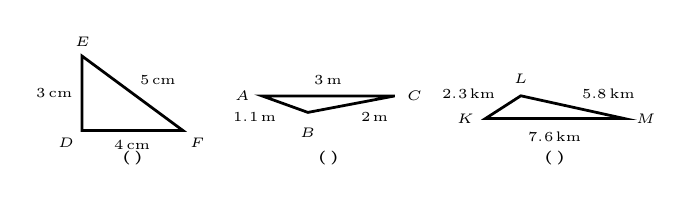
\begin{tikzpicture}[scale=0.61, every node/.style={font=\tiny, text=black}]
    % (1) DEF: 3, 4, 5
    \begin{scope}[shift={(0, 0)}]
      \coordinate (D) at (0,0); \coordinate (F) at (2.1,0); \coordinate (E) at (0,1.55);
      \draw[black, line width=1.0pt] (D)--(F)--(E)--cycle;
      \node[below left=-1pt] at (D) {$D$}; \node[above=0pt] at (E) {$E$}; \node[below right=-1pt] at (F) {$F$};
      \node[left=0pt] at (0,0.78) {$3\unit{cm}$};
      \node[below=0pt] at (1.05,0) {$4\unit{cm}$};
      \node[above right=-1pt] at (1.05,0.78) {$5\unit{cm}$};
      \node at (1.05,-0.58) {\textbf{(១)}};
    \end{scope}
    % (2) ABC: 1.1, 2, 3 (*0.92: A=(0,0), C=(2.76,0), B=(0.952,-0.343))
    \begin{scope}[shift={(3.75, 0.72)}]
      \coordinate (A) at (0,0); \coordinate (C) at (2.76,0); \coordinate (B) at (0.952,-0.343);
      \draw[black, line width=1.0pt] (A)--(B)--(C)--cycle;
      \node[left=1pt] at (A) {$A$}; \node[right=1pt] at (C) {$C$}; \node[below=2pt] at (B) {$B$};
      \node[above=0pt] at (1.38,0.02) {$3\unit{m}$};
      \node[below left=-1pt] at (0.45,-0.18) {$1.1\unit{m}$};
      \node[below right=-1pt] at (1.90,-0.18) {$2\unit{m}$};
      \node at (1.38,-1.30) {\textbf{(២)}};
    \end{scope}
    % (3) KLM: 2.3, 5.8, 7.6 (*0.38: K=(0,0), M=(2.888,0), L=(0.735,0.473))
    \begin{scope}[shift={(8.40, 0.25)}]
      \coordinate (K) at (0,0); \coordinate (M) at (2.888,0); \coordinate (L) at (0.735,0.473);
      \draw[black, line width=1.0pt] (K)--(L)--(M)--cycle;
      \node[left=1pt] at (K) {$K$}; \node[above=1pt] at (L) {$L$}; \node[right=1pt] at (M) {$M$};
      \node[above left=-1pt] at (0.36,0.24) {$2.3\unit{km}$};
      \node[above right=-1pt] at (1.85,0.24) {$5.8\unit{km}$};
      \node[below=1pt] at (1.44,-0.02) {$7.6\unit{km}$};
      \node at (1.44,-0.83) {\textbf{(៣)}};
    \end{scope}
  \end{tikzpicture}\par}

  \vspace{2pt}\hrule height 0.45pt\vspace{3pt}

  % --- លំហាត់ទី ១៤ (សៀវភៅទំព័រ ១៦៦ + កែតម្រូវ Erratum #4: 50° -> 60°) ---
  \fontsize{6.85pt}{9.4pt}\selectfont
  \textbf{លំហាត់ទី ១៤ (ទំ.១៦៦)៖} សរសេរ\textbf{ជ្រុង}តាមលំដាប់ពីវែងទៅខ្លី។ \textit{(\textbf{កែទំ.១៦៦៖} (៣) $\ang{G}=50^\circ$ [$170^\circ$] $\to \mathbf{60^\circ}$ [$180^\circ$]!)}\\[2pt]
  {\centering
  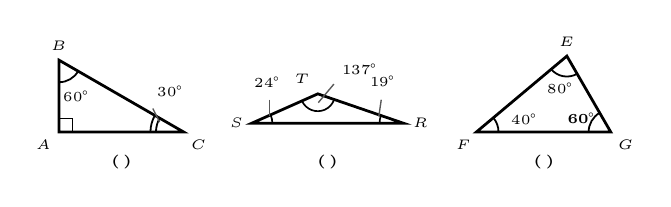
\begin{tikzpicture}[scale=0.62, every node/.style={font=\tiny, text=black}]
    % (1) ABC: 90, 60, 30 — labels strictly clear of lines (0 raw hits)
    \begin{scope}[shift={(0,0)}]
      \coordinate (A) at (0,0); \coordinate (C) at (2.55,0); \coordinate (B) at (0,1.47);
      \draw[black, line width=1.0pt] (A)--(B)--(C)--cycle;
      \pic[draw=black, line width=0.65pt, angle radius=1.7mm]{right angle=C--A--B};
      \pic[draw=black, line width=0.65pt, angle radius=2.8mm]{angle=A--B--C};
      \pic[draw=black, line width=0.65pt, angle radius=3.5mm]{angle=B--C--A};
      \pic[draw=black, line width=0.65pt, angle radius=4.2mm]{angle=B--C--A};
      \node[below left=-1pt] at (A) {$A$}; \node[above=0pt] at (B) {$B$}; \node[below right=-1pt] at (C) {$C$};
      \node at (0.36, 0.72) {$60^\circ$};
      \node[above right=1pt] at (1.78, 0.48) {$30^\circ$};
      \draw[darkline, line width=0.5pt] (1.92, 0.48) -- (2.06, 0.20);
      \node at (1.28,-0.62) {\textbf{(១)}};
    \end{scope}
    % (2) STR: 24, 137, 19 — clean external callout leaders (0 raw hits)
    \begin{scope}[shift={(3.95,0.18)}]
      \coordinate (S) at (0,0); \coordinate (R) at (3.10,0); \coordinate (T) at (1.35,0.60);
      \draw[black, line width=1.0pt] (S)--(T)--(R)--cycle;
      \pic[draw=black, line width=0.6pt, angle radius=2.6mm]{angle=R--S--T};
      \pic[draw=black, line width=0.6pt, angle radius=2.2mm]{angle=S--T--R};
      \pic[draw=black, line width=0.6pt, angle radius=3.0mm]{angle=T--R--S};
      \node[left=0pt] at (S) {$S$}; \node[above left=0.5pt] at (T) {$T$}; \node[right=0pt] at (R) {$R$};
      \node[above=1pt] at (0.32, 0.48) {$24^\circ$};
      \draw[darkline, line width=0.5pt] (0.36, 0.48) -- (0.36, 0.14);
      \node[above right=0pt] at (1.65, 0.78) {$137^\circ$};
      \draw[darkline, line width=0.5pt] (1.68, 0.80) -- (1.36, 0.42);
      \node[above=1pt] at (2.68, 0.48) {$19^\circ$};
      \draw[darkline, line width=0.5pt] (2.65, 0.48) -- (2.60, 0.14);
      \node at (1.55,-0.80) {\textbf{(២)}};
    \end{scope}
    % (3) FEG: 40, 80, 60 (Harmonized Erratum #4: 50 -> 60! 0 raw hits)
    \begin{scope}[shift={(8.55,0)}]
      \coordinate (F) at (0,0); \coordinate (G) at (2.75,0); \coordinate (E) at (1.852,1.554);
      \draw[black, line width=1.0pt] (F)--(E)--(G)--cycle;
      \pic[draw=black, line width=0.65pt, angle radius=2.8mm]{angle=G--F--E};
      \pic[draw=black, line width=0.65pt, angle radius=2.6mm]{angle=F--E--G};
      \pic[draw=black, line width=0.65pt, angle radius=2.8mm]{angle=E--G--F};
      \node[below left=-1pt] at (F) {$F$}; \node[above=0pt] at (E) {$E$}; \node[below right=-1pt] at (G) {$G$};
      \node at (0.98, 0.25) {$40^\circ$};
      \node at (1.72, 0.90) {$80^\circ$};
      \node at (2.15, 0.28) {$\mathbf{60^\circ}$};
      \node at (1.38,-0.62) {\textbf{(៣)}};
    \end{scope}
  \end{tikzpicture}\par}

  \vspace{2pt}\hrule height 0.45pt\vspace{3pt}

  % --- លំហាត់ទី ១៥ (សៀវភៅទំព័រ ១៦៦) ---
  \noindent
  \begin{minipage}[c]{5.20cm}
    \fontsize{6.85pt}{9.5pt}\selectfont
    \textbf{លំហាត់ទី ១៥ (ទំ.១៦៦)៖} $PQR$ ជាត្រីកោណមួយដែល $QR > QP$ និង $PR = PQ$ ។ បង្ហាញថា $\ang{P} > \ang{Q}$ ។\\
    {\fontsize{6.3pt}{8.8pt}\selectfont\textit{តម្រុយ៖} ប្រើ $QR>QP \Rightarrow \ang{P}>\ang{R}$ (\cnum{2}) និង $PR=PQ \Rightarrow \ang{Q}=\ang{R}$ $\Rightarrow \ang{P}>\ang{Q}$ (\cnum{5})!}
  \end{minipage}\hfill
  \begin{minipage}[c]{3.40cm}
    \centering
    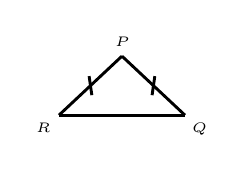
\begin{tikzpicture}[scale=0.50, every node/.style={font=\tiny, text=black}]
      \coordinate (R) at (0,0); \coordinate (Q) at (3.20,0); \coordinate (P) at (1.60,1.50);
      \draw[black, line width=1.05pt] (R)--(Q);
      \draw[black, line width=1.05pt, tkslash] (P)--(R);
      \draw[black, line width=1.05pt, tkslashR] (P)--(Q);
      \node[above=0pt] at (P) {$P$};
      \node[below left=-1pt] at (R) {$R$};
      \node[below right=-1pt] at (Q) {$Q$};
    \end{tikzpicture}
  \end{minipage}

  \vspace{3pt}
  \begin{tcolorbox}[
    enhanced, sharp corners, colback=panelgray, colframe=black,
    boxrule=0.7pt, boxsep=1pt, top=2.5pt, bottom=2.5pt, left=4pt, right=4pt
  ]
    \fontsize{6.25pt}{8.8pt}\selectfont
    \textbf{ផ្ទៀង (\cnum{1}--\cnum{5})៖}
    \chkbox~សំអាង \cnum{1}--\cnum{5} គ្រប់ \en{|} \chkbox~លេខ ១៣(២) \en{|} \chkbox~កែ ១៤(៣) $\to 60^\circ$!
  \end{tcolorbox}
\end{tcolorbox}%
}

\noindent
\hwslipFourINEQ{ប័ណ្ណទី ១}\hfill\hwslipFourINEQ{ប័ណ្ណទី ២}

\vspace{7pt}
\noindent\scissors\ \dotfill\ \textbf{កាត់តាមស្នាមចុចចែកជា ៤ ប័ណ្ណ (\en{Cut Along Dashed Lines})} \dotfill\ \scissors
\vspace{7pt}

\noindent
\hwslipFourINEQ{ប័ណ្ណទី ៣}\hfill\hwslipFourINEQ{ប័ណ្ណទី ៤}

\end{document}
